\chapter{Goniometria}
\label{sec:GONIOMETRIA}
\minitoc
\mtcskip                                % put some skip here
\minilof                                % a minilof
\mtcskip                                % put some skip here
\minilot
\section{Angoli}
\label{sec:gonioang}
\begin{definizione}[Angolo]
Un angolo\index{Angolo} è la parte di piano compreso fra due semirette dette lati hanno in comune l'origine chiamata vertice.
\end{definizione}

Le  semirette formano due angoli  uno convesso\index{Angolo!convesso} l'altro concavo\index{Angolo!concavo} come nella figura\nobs\vref{fig:angconconvposoneg}. 
\begin{figure} %[htbp]
	\centering
	\begin{tikzpicture}[>=triangle  45,x=1.5cm,y=1.5cm]
	\coordinate (C) at (0,0);
	\coordinate (A) at (1.5,1.5);
	\coordinate (B) at (-2,0);
	\matrix[column sep=0.8cm,row sep=0.5cm]{
		\draw (A) - -(C);
		\draw (B) - -(C);
		\draw [<->] (1,1) arc(45:180:2cm);
		\draw [<->, dashed,] (-1.25,0)  arc(-180:45:2cm);
		\node (A1) at (0,2) {\textbf{{\Large Angolo convesso}}};
		\node (A2) at (0,-2) {\textbf{{\Large Angolo concavo}}};
		\node[draw, circle, inner sep=.3mm] (a) at (C) {};&
		\draw (A) - -(C);
		\draw (B) - -(C);
		\draw [->] (1,1) arc(45:180:2cm);
		\draw [<-, dashed,] (-1.25,0)  arc(-180:45:2cm);
		\node (A1) at (0,2) {\textbf{{\Large Angolo positivo}}};
		\node (A2) at (0,-2) {\textbf{{\Large Angolo negativo}}}; 
		\node[draw, circle, inner sep=.3mm] (a) at (C) {};
		\\  
	};
	\end{tikzpicture}
	\caption{Angoli concavi e convessi, positivi e negativi}
	\label{fig:angconconvposoneg}
\end{figure}
\begin{figure} %[htbp]
	\centering
	\begin{tikzpicture}[>=triangle  45,x=1.5cm,y=1.5cm]
	\coordinate (C) at (0,0);
	\coordinate (A) at (1.,0);
	\coordinate (B) at (-2,0);
	\coordinate (AA) at (-0.5,-1.5);
	\coordinate (DD) at (-1,-1.5);
	\coordinate (EE) at (1,-1.5);
	\coordinate (FF) at (-1,0);
	\coordinate (CC) at (-0.5,0);
	\matrix[column sep=0.8cm,row sep=1cm]{
		\draw (AA) - -(CC);
		\draw (A) - -(CC);
		\draw [<-] (-0.5,-1) arc(-90:0:1);
		\node (A2) at (-1,-2) {\textbf{{Angolo retto negativo}}}; 
		\node[draw, circle, inner sep=.3mm] (a) at (CC) {};
		&
		\draw (EE) - -(DD);
		\draw (FF) - -(DD);
		\draw [<-] (-1,-.5) arc(90:0:1);
		\node (A2) at (-1,-2) {\textbf{{Angolo retto positivo}}}; 
		\node[draw, circle, inner sep=.3mm] (a) at (DD) {};\\
		\draw (A) - -(C);
		\draw (B) - -(C);
		\draw [<-] (-0.0,0) arc(0:180:0.5);
		\node (A1) at (-1,-1) {\textbf{{ Angolo piatto negativo}}};
		\node[draw, circle, inner sep=.3mm] (a) at (-0.4,0) {};
		&
		\draw (A) - -(C);
		\draw (B) - -(C);
		\draw [->] (-0.0001,0) arc(0:180:0.5);
		\node (A1) at (-1,-1) {\textbf{{ Angolo piatto positivo}}};
		\node[draw, circle, inner sep=.3mm] (a) at (-0.4,0) {};\\ 
		\draw (-.4,0) - -(1,0);
		\draw [<-] (.5,0) arc(0:360:1);
		\node (A1) at (-1,-2) {\textbf{{ Angolo giro negativo}}};
		\node[draw, circle, inner sep=.3mm] (a) at (-0.4,0) {};
		&
		\draw (-.4,0) - -(1,0);
		\draw [->] (.5,0) arc(0:360:1);
		\node (A1) at (-1,-2) {\textbf{{ Angolo giro positivo}}};
		\node[draw, circle, inner sep=.3mm] (a) at (-0.4,0) {};\\
		&
		\draw (-1,0) - -(0.,0);
		\node (A1) at (-1,-1) {\textbf{{ Angolo nullo}}};
		\node[draw, circle, inner sep=.3mm] (a) at (-1,0) {};\\
	};
	\end{tikzpicture}
	\caption{Angoli notevoli}
	\label{fig:Angolorettoposneggonio}
\end{figure}
\begin{figure}
	\begin{tikzpicture}[>=latex',line join=bevel,scale=0.8]
	%%
	\node (11) at (392.29bp,17.829bp) [draw,ellipse] {Verso  orario};
	\node (10) at (388.16bp,74.845bp) [draw,draw=none] {ha};
	\node (13) at (70.905bp,76.517bp) [draw,draw=none] {ha};
	\node (12) at (141.61bp,19.288bp) [draw,ellipse] {Positivo};
	\node (15) at (250.05bp,136.65bp) [draw,draw=none] {è};
	\node (14) at (27.065bp,155.97bp) [draw,ellipse] {Verso antiorario};
	\node (17) at (234.48bp,30.164bp) [draw,ellipse] {Convesso};
	\node (16) at (156bp,165.7bp) [draw,ellipse] {Concavo};
	\node (1) at (228.45bp,186.28bp) [draw,ellipse] {Angolo};
	\node (3) at (415.46bp,231.25bp) [draw,ellipse] {un'ampiezza};
	\node (2) at (325.1bp,199.22bp) [draw,draw=none] {ha};
	\node (5) at (204.94bp,325.19bp) [draw,ellipse] {una parte di piano};
	\node (4) at (186.96bp,277.36bp) [draw,draw=none] {è};
	\node (7) at (323.86bp,353.56bp) [draw,ellipse] {fra due semirette};
	\node (6) at (291.86bp,301.26bp) [draw,draw=none] {compreso};
	\node (9) at (300.59bp,83.181bp) [draw,ellipse] {Negativo};
	\node (8) at (193.44bp,87.52bp) [draw,draw=none] {è};
	\draw [->] (5) ..controls (237.78bp,316.15bp) and (246.42bp,313.77bp)  .. (6);
	\draw [->] (15) ..controls (245bp,102.07bp) and (241.38bp,77.363bp)  .. (17);
	\draw [->] (2) ..controls (361.57bp,212.14bp) and (372.16bp,215.9bp)  .. (3);
	\draw [->] (6) ..controls (304.69bp,322.24bp) and (306.41bp,325.04bp)  .. (7);
	\draw [->] (1) ..controls (236.69bp,167.34bp) and (237.39bp,165.72bp)  .. (15);
	\draw [->] (15) ..controls (212.73bp,148.18bp) and (201.12bp,151.76bp)  .. (16);
	\draw [->] (4) ..controls (194.09bp,296.32bp) and (194.43bp,297.21bp)  .. (5);
	\draw [->] (13) ..controls (55.177bp,105.02bp) and (47.793bp,118.4bp)  .. (14);
	\draw [->] (9) ..controls (334.75bp,79.929bp) and (342.94bp,79.149bp)  .. (10);
	\draw [->] (1) ..controls (214.5bp,216.9bp) and (206.27bp,234.97bp)  .. (4);
	\draw [->] (12) ..controls (117.28bp,38.976bp) and (109.22bp,45.501bp)  .. (13);
	\draw [->] (1) ..controls (216.93bp,153.78bp) and (209.31bp,132.31bp)  .. (8);
	\draw [->] (1) ..controls (265.19bp,191.2bp) and (276.86bp,192.76bp)  .. (2);
	\draw [->] (8) ..controls (173.61bp,61.419bp) and (166.59bp,52.179bp)  .. (12);
	\draw [->] (8) ..controls (233.42bp,85.901bp) and (249.13bp,85.265bp)  .. (9);
	\draw [->] (10) ..controls (389.72bp,53.373bp) and (389.98bp,49.706bp)  .. (11);
	%
	\end{tikzpicture}
	\caption{Mappa goniometria l'angolo}
	\label{fig:MappaGonometria1}
\end{figure}
\begin{definizione}[Angoli Positivi e Negativi]
	Fissato un lato, l'angolo è  positivo\index{Angolo!positivo}  se per costruirlo ruoteremo l'altra semiretta in senso antiorario.  Un angolo è negativo\index{Angolo!negativo} se ruoteremo l'altro lato in senso orario come nella figura\nobs\vref{fig:angconconvposoneg}. ...
\end{definizione}
\begin{definizione}[Angolo giro]
Un angolo è giro\index{Angolo!giro} quando le due semirette coincidono. 
\end{definizione}
\begin{definizione}[Angolo piatto]
Un angolo è  piatto\index{Angolo!retto} quando i suoi lati  coincidono con la stessa retta.
\end{definizione}
\begin{definizione}[Angolo retto]
Avremo un angolo è retto\index{Angolo!retto} quando è la metà di un angoli piatto. 
\end{definizione}
\begin{definizione}[Angolo acuto]
Un angolo è acuto\index{Angolo!acuto} se  minore di un  retto.
\end{definizione}
\begin{definizione}[Angolo ottuso]
Un angolo è ottuso\index{Angolo!ottuso} se  maggiore di un  retto.
\end{definizione}
 La figura\nobs\vref{fig:Angolorettoposneggonio} mostra  vari casi
\section{Misura dell'angolo}
\label{sec:MisuraAngoloGonio}

A ogni angolo viene associata una grandezza detta ampiezza.  Per misurare l'ampiezza dell'angolo si usa o il grado sessagesimale  o i radianti
\subsection{Angolo sessagesimale}
\begin{definizione}[Grado]
Un grado\index{Grado} è la trecentosessantesima parte in un angolo giro. Il grado si suddivide in minuti e  secondi. Il minuto è la sessantesima parte di un grado. Il secondo è la sessantesima parte di un minuto. Il secondo è suddiviso in decimi e centesimi.
\end{definizione}
 Quindi \[\ang{;1;}=\dfrac{\ang{1}}{60}\] e  \[\ang{;;1}=\dfrac{\ang{;1;}}{60}=\dfrac{\ang{1}}{3600}\]
\begin{esempio}
L'angolo  \ang{45;30;20}  ha l'ampiezza di \ang{45} gradi \ang{;30;} minuti e \ang{;;20} secondi. L'angolo \ang{30;45;23,7} secondo ha l'ampiezza di \ang{30} gradi \ang{;45;} minuti e \ang{;;23} secondi e $7$ decimi.
\end{esempio}
Un angolo giro\index{Angolo!giro} è quindi ampio \ang{360} gradi. L'angolo piatto\index{Angolo!piatto},  metà di un angolo giro, ha l'ampiezza di \ang{180} gradi. L'angolo retto\index{Angolo!retto}  metà di una angolo piatto, ha ampiezza di \ang{90} gradi.

Un angolo espresso in gradi sessagesimali può essere scritto in forma decimale. 
\begin{esempio}
 Abbiamo un angolo di ampiezza pari a \ang{44;58;48} e vogliamo scriverlo in forma decimale.   Dato che $\ang{;1;}=\dfrac{\ang{1}}{60}$ e che $\ang{;;1}=\dfrac{\ang{;1;}}{60}=\dfrac{\ang{1}}{3600}$  avremo
\begin{align*}
	\ang{44;58;48}&=\ang{44}+\left(\dfrac{58}{60}\right)^{\circ}+\left(\dfrac{48}{3600} \right)^{\circ}\\
	&=\ang{44}+\left(\dfrac{29}{30}\right)^{\circ}+\left(\dfrac{3}{225} \right)^{\circ}\\
	&=\ang{44}+\left(\dfrac{6+435}{450} \right)^{\circ}\\
	&=\ang{44}+\left(\dfrac{441}{450} \right)^{\circ}\\
	&=\ang{44}+\num{0,98}^{\circ}\\
	&=\num{44,98}^{\circ}
\end{align*}
\end{esempio}
\begin{esempio}
Convertiamo $7,42^{\circ}$ in gradi minuti e secondi:
\begin{align*}
	7,42^{\circ}&=7^{\circ}+0,42^{\circ}\\
	&=\ang{7}+0,42\cdot \ang{1}\\
	&=\ang{7}+0,42\cdot \ang{;60;}\\
	&=\ang{7;25,2;}\\
	&=\ang{7;25;}+\ang{;0,2;}\\
	&=\ang{7;25;}+0,2\cdot\ang{;1;}\\
	&=\ang{7;25;}+0,2\cdot\ang{;;60}\\
	&=\ang{7;25;12}\\
\end{align*} 
\end{esempio}
\subsection{Radianti}
\begin{definizione}[Radiante]
Data una circonferenza di raggio $r$ e  un angolo $\alpha$ con il vertice nel centro $C$ della circonferenza, come nella figura\nobs\vref{fig:radinatidefgonio}. Se $l$ è la lunghezza dell'arco di circonferenza sotteso dall'angolo, chiamo radiante il rapporto \[\rho=\dfrac{l}{r} \]
\end{definizione}

Avremo quindi che un angolo ha l'ampiezza di un radiante\index{Radiante} se l'arco di circonferenza $l$ è uguale al raggio $r$.

In un angolo giro\index{Angolo!giro} l'arco è lungo quanto la circonferenza. La sua misura in radianti è \[\rho=\dfrac{2\pi r}{r}=2\pi\]. 

Un angolo piatto, meta di un giro,  misura  \[\rho=\pi\]\index{Angolo!piatto} e  un angolo retto\index{Angolo!retto} misura \[\rho=\dfrac{\pi}{2} \] 

Per convertire  da gradi sessagesimali a radianti si procede in questo modo:
\begin{align*}
\dfrac{l}{2\pi r}&=\dfrac{\alpha}{\ang{360}}\\
\dfrac{\rho}{2\pi}&=\dfrac{\alpha}{\ang{360}}\\
\rho&=\dfrac{\alpha 2\pi}{\ang{360}}\\
\rho&=\dfrac{\alpha\pi}{\ang{180}}
\end{align*}
segue che per passare da radianti a gradi sessagesimali avremo\[\alpha=\dfrac{\ang{180}}{\pi}\rho \]
\begin{figure}
	\centering
	\begin{tikzpicture}[>=triangle  45,x=1.5cm,y=1.5cm]
	\pgfmathsetmacro{\raggio}{2};
	\coordinate [label=below:$O$] (C) at (0,0);
	\coordinate (A) at (1.8,2);
	\coordinate (B) at (2,0);
	\draw[name path=cc] (C) circle (\raggio);
	\path [name path=C--A] (C) -- (A);
	\path [name path=C--B] (C) -- (B);
	\draw [name intersections={of=cc and C--B,by=M}] (C) -- (M) node[above right]{$A$};
	\draw [name intersections={of=cc and C--A,by=N}] (C) -- (N) node[above]{$B$};
	\node(arco)at($(M)!0.5!(N)$){$\displaystyle l$};
	\node(raggio)at($(C)!0.5!(B)$) [label=below:$\displaystyle r$]{};
	\node(angolo)at(0.3,.3) [label=right:$\alpha$] {};
	\draw [->] (1,0) arc(0:48:1);
	\end{tikzpicture}
	\caption{Radianti}
	\label{fig:radinatidefgonio}
\end{figure}
\section{Funzioni goniometriche}
\label{sec:FunzioniGoniometriche}
\begin{definizione}[Circonferenza goniometrica]
	Dato un sistema di riferimento cartesiano ortogonale, una circonferenza goniometrica\index{Circonferenza!goniometrica} è una circonferenza con centro nell'origine e raggio uguale a uno. 
\end{definizione}
\begin{figure}
	\centering
	\begin{tikzpicture}[>=triangle  45,x=1.5cm,y=1.5cm]
	\pgfmathsetmacro{\raggio}{2};
	\coordinate (C) at (0,0);
	\coordinate (A) at (1.8,2);
	\coordinate (B) at (2,0);
	\draw[name path=cc] (C) circle (\raggio);
	\path [name path=C--A] (C) -- (A);
	\path [name path=C--B] (C) -- (B);
	\draw [name intersections={of=cc and C--B,by=M}] (C) -- (M) node[above right]{$A$};
	\draw [name intersections={of=cc and C--A,by=N}] (C) -- (N) node[above]{$P$};
	\node(angolo)at(0.3,.3) [label=right:$\alpha$] {};
	\node(OO)at(-0.5,-.2) [label=right:$O$] {};
	\node(AA)at(-0.1,2.1) [label=right:$B$] {};
	\node(BB)at(-0.1,-2.1) [label=right:$D$] {};
	\node(CC)at(-2.4,.12) [label=right:$C$] {};	
	\draw [->] (1,0) arc(0:48:1);
	\draw[->](-2.5,0)--(2.5,0);
	\draw[->](0,-2.5)--(0,2.5);
	\end{tikzpicture}
	\caption{Circonferenza goniometrica}
	\label{fig:circonferenzagonimetricagonio}
\end{figure}
 La circonferenza incontra gli assi in quattro punti. $A(1,0)$, $B(0,1)$, $C(-1,0)$ e $D(-1,0)$. Costruiamo un angolo  $\alpha$  in modo che il suo vertice coincida con il centro della circonferenza. L'angolo incontra la circonferenza nei punti $A$ e $P$ come nella  figura\nobs\vref{fig:circonferenzagonimetricagonio}. 
\subsection{Coseno}
\label{sec:cosenogonio}
\begin{figure}
	\begin{subfigure}[b]{.5\linewidth}
		\centering	\begin{tikzpicture}[>=triangle  45,scale=0.5]
		\tikzset{samples=600}
		\pgfmathsetmacro{\raggio}{3};
		\pgfmathsetmacro{\angolo}{60};
		\pgfmathsetmacro{\y}{3};
		\pgfmathsetmacro{\XM}{\raggio};
		\pgfmathsetmacro{\sraggio}{1.9*\raggio};
		\coordinate [label=below left:$O$] (oo)  at (0,0);
		\draw[->] (-\raggio-1,0) -- (\raggio+1,0) node[above] {$x$} ;
		\draw[->] (0,-\raggio-1) -- (0,\raggio+1) node[above] {$y$} ;
		\draw (oo) circle (\raggio) ;
		
		\coordinate[label=above:$P$] (P) at ({\raggio*cos(\angolo)},{\raggio*sin(\angolo )});
		
		\coordinate [label=below right:$Q$] (Q) at ($((-\raggio,0)!(\angolo:\raggio)!(\raggio,0)$);
		\coordinate [label=below  :$\cos\alpha$] (M) at ($(Q)!0.5!(oo)$);
		\draw[->] (\sraggio/\y,0 ) arc (0:\angolo:\sraggio/\y) node[ right=7pt] {$\alpha$};
		\draw (oo)-- (P) ;
		\draw[dashed](Q)-- (P) ;		
		\end{tikzpicture}
		\caption{Coseno definizione}\label{sub:cosenodef}
	\end{subfigure}%
	\begin{subfigure}[b]{.5\linewidth}
		%\centering\includegraphics[scale=0.34]{cosenografico-crop}
		\centering
		\begin{tikzpicture}[>=triangle  45,scale=0.5]
		\tikzset{samples=600}
		\pgfmathsetmacro{\a}{3};
		\pgfmathsetmacro{\Xm}{-2*pi};
		\pgfmathsetmacro{\XM}{2*pi};
		\coordinate (A) at (-5/4*pi,{\a*cos(-5/4*pi r)});
		\coordinate (B) at (3/4*pi,{\a*cos(3/4*pi r)});
		\node (C )at (0,\a)[above left] {$1$};
		\node (D )at (0,-\a)[above left] {$-1$};
		\coordinate (A) at (-5/4*pi,{\a*cos(-5/4*pi r)});
		\coordinate (B) at (3/4*pi,{\a*cos(3/4*pi r)});
		\draw[->] (\Xm,0) -- (\XM,0) node[above] {$\alpha$} ;
		\draw[->] (0,-\a-1) -- (0,\a+1) node[above] {$\cos\alpha$} ;;
		\draw (\Xm,\a) -- (\XM,\a) ;
		\draw (\Xm,-\a) -- (\XM,-\a) ;
		\draw [thick, domain=\Xm:\XM] plot  (\x,{\a*cos(\x r)});  \
		\draw[dashed] (A)-- (B) ;  
		\end{tikzpicture}
		\caption{Coseno grafico}\label{sub:cosenograf}
	\end{subfigure}
	\caption{Coseno}
	\label{tab:funzcos}
\end{figure}
\begin{definizione}[Coseno]
Data una circonferenza goniometrica\nobs\vref{sub:cosenodef}, disegno un angolo con centro nell'origine e di ampiezza $\alpha$. Un lato dell'angolo incontra la circonferenza in un punto $P$.  Chiamo coseno\index{Funzione!Coseno!definizione} dell'angolo $\alpha$ e lo indico con $\cos\alpha$ l'ascissa del punto $P$.
\end{definizione}
\subsection{Andamento coseno}
\label{sec:andamentocoseno}
Al variare dell'angolo varia anche il valore del coseno\index{Funzione!Coseno}, consideriamo la figura\nobs\vref{fig:AndamentoCoseno1}. Supponiamo di far variare l'angolo $\alpha$ da zero a centottanta gradi, quindi che $\ang{0}\leq\alpha\leq\ang{180}$ o se utilizziamo i radianti $0\leq\alpha\leq\pi$. 
\begin{description}
	\item[$\alpha_0$] L'angolo ha ampiezza zero. La verticale del punto $P_0$ all'asse $x$ lo incontra in $px_0$. In questo caso il coseno di $\alpha$ cioè $\cos\alpha_0$ vale uno.
	\item [$\alpha_1$] l'angolo è compreso fra zero e novanta gradi, incontra la circonferenza nel punto $P_1$. La sua verticale incontra l'asse delle ascisse nel punto $px_1$. Il coseno dell'angolo $\alpha_1$ è un numero positivo minore di uno.
	\item [$\alpha_2$] L'angolo  è retto. La proiezione del punto $P_2$ incontra l'asse $x$ nell'origine. In questo caso l'ascissa è $x_2$ è   nulla e $\cos\alpha_2$ è zero. 
	\item [$\alpha_3$]  L'angolo è ottuso. La proiezione del punto $P_3$ incontra  l'asse $x$ nel semiasse negativo. Quindi $\cos\alpha_2$ è negativo.
	\item [$\alpha_4$] L'angolo  è  piatto. Il  $P_4$ incontra l'asse $x$ nel punto $(-1;0)$. In questo  $\cos\alpha_4$ vale meno uno.
\end{description}
Analogo discorso per angoli di ampiezza  maggiore di un angolo  piatto come nella figura~\vref{fig:AndamentoCoseno2}.
\begin{description}
	\item [$\alpha_4$] L'angolo è piatto. Il  $P_4$ incontra l'asse $x$ nel punto $(-1;0)$. In questo  $\cos\alpha_4$ vale meno uno.
	\item [$\alpha_5$] L'angolo è compreso tra \ang{180} e \ang{270}. La proiezione del punto $P_5$ cade sul semiasse negativo delle ascisse. Quindi $\cos\alpha_2$ è negativo.
	\item [$\alpha_6$] L'angolo è di duecentosettanta gradi. Il punto ha ascissa zero quindi  $\cos\alpha_6=0$.
	\item [$\alpha_7$] L'angolo è compreso tra \ang{180} e \ang{360}. La proiezione del punto $P_7$ cade sul semiasse positivo delle ascisse. Quindi $\cos\alpha_7$ è positivo.
	\item [$\alpha_8$] L'angolo è di trecentosessanta gradi. Il punto ha ascissa uno quindi  $\cos\alpha_8=1$.
\end{description}
Per angoli superiori a \ang{360} otteniamo gli stessi casi illustrati in precedenza. 
Possiamo quindi dire che il coseno
\begin{enumerate}
	\item è limitato e varia fra $-1$ e $+1$.
	\item è periodico, di periodo pari a \ang{360} o $2\pi$
	\end{enumerate} 
\begin{figure}
		\centering
		\begin{tikzpicture}[>=triangle  45,scale=0.8] %, x=0.8cm,y=0.8cm]
		% draw the coordinates
		\pgfmathsetmacro{\raggio}{4};
		\pgfmathsetmacro{\mraggio}{\raggio/3};
		\pgfmathsetmacro{\qraggio}{\raggio/5};
		\pgfmathsetmacro{\sraggio}{1.9*\raggio};
		% draw the unit circle
		\draw[->] (0,-\raggio-\mraggio) -- (0,\raggio+\mraggio+0.5) node[above,fill=white] {$y$};
		\draw[->] (-\raggio-\mraggio,0) -- (\raggio+\mraggio,0) node[right,fill=white] {$x$};
		\draw[thick] (0,0) circle(\raggio);
		%\draw (-\raggio-\qraggio-0.2,0) node[above=1pt] {$(-1,0)$}
		%(\raggio+\qraggio,0)  node[above=1pt] {$(1,0)$}
		%(0,-\raggio-\qraggio-0.2) node[fill=white] {$(0,-1)$}
		%(0,\raggio+\qraggio+0.2)  node[fill=white] {$(0,1)$};
		\node(OO)at(0,0) [label= below right:$O$] {};
		\foreach \x in {180,240,270,300,360}{
			% lines from center to point
			\draw[gray] (0,0) -- (\x:\raggio);
			% dots at each point
			\filldraw[black] (\x:\raggio) circle(2pt);
			% draw each angle in degrees
			%\draw (\x:0.8*\raggio) node[fill=white] {$\x^\circ$};
			\draw(\x:\raggio)--($((-1,0)!(\x:\raggio)!(1,0)$);
			\filldraw[black] ($((-1,0)!(\x:\raggio)!(1,0)$) circle(2pt);
		}
		\foreach \x/ \y/\arco  in {
			180/2.5/{\alpha_4},
			240/3/{\alpha_5},
			270/4/{\alpha_6},
			300/5/{\alpha_7},
			%150/6,
			360/7 /{\alpha_8}%,
			%210/8,
			%240/9,
			%270/10,
			%300/11,
			%330/12,
			%360/13
		}
		\draw[->] (\sraggio/\y,0 ) arc (0:\x:\sraggio/\y) node[above  =-20pt] {$\arco$};
		
		\foreach \x/ \y in {
			180/ px_4,	
			%30/px_1,	
			240/px_5,
			270/px_6,
			300/px_7,
			%150/px_5,
			360/px_8	 %,
			%210/8,
			%240/9,
			%270/10,
			%300/11,
			%330/12,
			%360/13
		}
		\draw ($((-1,0)!(\x:\raggio)!(1,0)$) node[above=4pt] {$\y$};
		\foreach \x/ \y in {
			180/ P_4,	
			%30/P_1,	
			240/P_5,
			270/P_6,
			300/P_7,
			%150/P_8,
			360/P_8 %,
			%210/8,
			%240/9,
			%270/10,
			%300/11,
			%330/12,
			%360/13
		}
		\draw ( \x:\raggio) node[above  left =-21pt] {$\y$};
		\end{tikzpicture}
		\caption{Andamento coseno $\ang{0}<\alpha<\ang{180}$}\label{fig:AndamentoCoseno1}
	\end{figure}%
	\begin{figure}
		\centering
\begin{tikzpicture}[>=triangle  45,scale=0.8] %, x=0.8cm,y=0.8cm]
% draw the coordinates
\pgfmathsetmacro{\raggio}{4};
\pgfmathsetmacro{\mraggio}{\raggio/3};
\pgfmathsetmacro{\qraggio}{\raggio/5};
\pgfmathsetmacro{\sraggio}{1.9*\raggio};
% draw the unit circle
\draw[->] (0,-\raggio-\mraggio) -- (0,\raggio+\mraggio+0.5) node[above] {$y$};
\draw[->] (-\raggio-\mraggio,0) -- (\raggio+\mraggio,0) node[right] {$x$};
\draw[thick] (0,0) circle(\raggio);
%\draw (-\raggio-\qraggio-0.2,0) node[above=1pt] {$(-1,0)$}
%(\raggio+\qraggio,0)  node[above=1pt] {$(1,0)$}
%(0,-\raggio-\qraggio-0.2) node[fill=white] {$(0,-1)$}
%(0,\raggio+\qraggio+0.2)  node[fill=white] {$(0,1)$};
\node(OO)at(0,0) [label= below right:$O$] {};
\foreach \x in {180,240,270,300,360}{
	% lines from center to point
	\draw[gray] (0,0) -- (\x:\raggio);
	% dots at each point
	\filldraw[black] (\x:\raggio) circle(2pt);
	% draw each angle in degrees
	%\draw (\x:0.8*\raggio) node[fill=white] {$\x^\circ$};
	\draw(\x:\raggio)--($((-1,0)!(\x:\raggio)!(1,0)$);
	\filldraw[black] ($((-1,0)!(\x:\raggio)!(1,0)$) circle(2pt);
}
\foreach \x/ \y/\arco  in {
	180/2.5/{\alpha_5},
	240/3/{\alpha_6},
	270/4/{\alpha_7},
	300/5/{\alpha_8},
	%150/6,
	360/7 /{\alpha_9}%,
	%210/8,
	%240/9,l
	%270/10,
	%300/11,
	%330/12,
	%360/13
}
\draw[->] (\sraggio/\y,0 ) arc (0:\x:\sraggio/\y) node[above  =-20pt] {$\arco$};

\foreach \x/ \y in {
	180/ px_5,	
	%30/px_1,	
	240/px_6,
	270/px_7,
	300/px_8,
	%150/px_5,
	360/px_9	 %,
	%210/8,
	%240/9,
	%270/10,
	%300/11,
	%330/12,
	%360/13
}
\draw ($((-1,0)!(\x:\raggio)!(1,0)$) node[above left=2pt] {$\y$};
\foreach \x/ \y in {
	180/ P_5,	
	%30/P_1,	
	240/P_6,
	270/P_7,
	300/P_8,
	%150/P_5,
	360/P_9	 %,
	%210/8,
	%240/9,
	%270/10,
	%300/11,
	%330/12,
	%360/13
}
\draw ( \x:\raggio) node[above  =-21pt] {$\y$};
\end{tikzpicture}
		\caption{Andamento coseno $\ang{180}<\alpha<\ang{360} $}\label{fig:AndamentoCoseno2}
\end{figure}
\subsection{Seno}
\label{sec:senogonio}
\begin{figure}
	\begin{subfigure}[b]{.5\linewidth}
		%\centering\includegraphics[scale=0.35]{senoalpha-crop}
		\centering
			\begin{tikzpicture}[>=triangle  45,scale=0.5]
				\tikzset{samples=600}
				\pgfmathsetmacro{\raggio}{3};
				\pgfmathsetmacro{\angolo}{40};
				\pgfmathsetmacro{\y}{3};
				\pgfmathsetmacro{\XM}{\raggio};
				\pgfmathsetmacro{\sraggio}{1.9*\raggio};
				\coordinate [label=below left:$O$] (oo)  at (0,0);
				\draw[->] (-\raggio-1,0) -- (\raggio+1,0) node[above] {$x$} ;
				\draw[->] (0,-\raggio-1) -- (0,\raggio+1) node[above] {$y$} ;
				\draw (oo) circle (\raggio) ;
			
				\coordinate[label=above:$P$] (P) at ({\raggio*cos(\angolo)},{\raggio*sin(\angolo )});
				
				\coordinate [label=above left:$Q$] (Q) at ($((0,-\raggio)!(\angolo:\raggio)!(0,\raggio)$);
				\coordinate [label=above left :$\sen\alpha$] (M) at ($(Q)!0.5!(oo)$);
				\draw[->] (\sraggio/\y,0 ) arc (0:\angolo:\sraggio/\y) node[ right=3pt] {$\alpha$};
				\draw (oo)-- (P) ;
				\draw[dashed](Q)-- (P) ;		
		\end{tikzpicture}
		\caption{Seno definizione}\label{sub:senodef}
	\end{subfigure}%
	\begin{subfigure}[b]{.5\linewidth}
		\centering
		\begin{tikzpicture}[>=triangle  45,scale=0.5]
		\tikzset{samples=600}
		\pgfmathsetmacro{\a}{3};
		\pgfmathsetmacro{\Xm}{-2*pi};
		\pgfmathsetmacro{\XM}{2*pi};
		\coordinate [label=above left:$o$] (oo)  at (0,0);
		\coordinate (A) at (-5/4*pi,{\a*sin(-5/4*pi r)});
		\coordinate (B) at (3/4*pi,{\a*sin(3/4*pi r)});
		\node (C )at (0,\a)[above right] {$1$};
		\node (D )at (0,-\a)[above right] {$-1$};
		
		\draw[->] (\Xm,0) -- (\XM,0) node[above] {$\alpha$} ;
		\draw[->] (0,-\a-1) -- (0,\a+1) node[above] {$\sen\alpha$} ;;
		\draw (\Xm,\a) -- (\XM,\a) ;
		\draw (\Xm,-\a) -- (\XM,-\a) ;
		\draw [thick, domain=\Xm:\XM] plot  (\x,{\a*sin(\x r)});  
		\draw[dashed] (A)-- (B) ;  
		\end{tikzpicture}
		\caption{Seno grafico}\label{sub:senograf}
	\end{subfigure}
	\caption{Seno}
	\label{tab:funseno}
\end{figure}
\begin{definizione}[Seno]
	Data una circonferenza goniometrica\nobs\vref{sub:senodef}, disegno un angolo con centro nell'origine e di ampiezza $\alpha$. Un lato dell'angolo incontra la circonferenza in un punto $P$.  Chiamo seno\index{Funzione!Seno!definizione} dell'angolo $\alpha$ e lo indico con $\sen\alpha$ l'ordinata $OQ$  del punto $P$
\end{definizione}
\subsection{Andamento seno}
\label{subs:AndamentoSeno}
Al variare dell'angolo varia anche il valore del seno\index{Funzione!Seno}, consideriamo la figura\nobs\vref{fig:AndamentoSeno1}. Supponiamo di far variare l'angolo $\alpha$ da zero a centottanta gradi, quindi che $\ang{0}\leq\alpha\leq\ang{180}$ o se utilizziamo i radianti $0\leq\alpha\leq\pi$. 
\begin{description}
	\item[$\alpha_0$] L'angolo ha ampiezza zero. La verticale del punto $P_0$  incontra l'asse delle ordinate in $py_0$. In questo caso il seno di $\alpha$ cioè $\sen\alpha_0$ vale zero.
	\item [$\alpha_1$] l'angolo è compreso fra zero e novanta gradi, incontra la circonferenza nel punto $P_1$. La sua verticale incontra l'asse delle ordinate nel punto $py_1$. Il seno dell'angolo $\alpha_1$ è un numero positivo minore di uno.
	\item [$\alpha_2$] L'angolo  è retto. L'ordinata del punto $P_2$ è uno. In questo caso  è   $\sen\alpha_2$ è uno. 
	\item [$\alpha_3$]  L'angolo è ottuso. La perpendicolare del punto $P_3$ incontra  l'asse $y$ nel semiasse positivo. Quindi $\sen\alpha_2$ è maggiore di zero.
	\item [$\alpha_4$] L'angolo  è  piatto. Il  $P_4$ incontra l'asse $y$ nel punto $(-1;0)$. In questo  $\sen\alpha_4$ vale meno zero.
\end{description}
Analogo discorso per angoli di ampiezza  maggiore di un angolo  piatto come nella figura~\vref{fig:AndamentoSeno2}.
\begin{description}
	\item [$\alpha_4$] L'angolo è piatto. Il  $P_4$ incontra l'asse delle ordinate nel punto $(-1;0)$. In questo  $\sen\alpha_4$ vale zero.
	\item [$\alpha_5$] L'angolo è compreso tra \ang{180} e \ang{270}. La proiezione del punto $P_5$ cade sul semiasse negativo delle ordinate. Quindi $\sen\alpha_2$ è negativo.
	\item [$\alpha_6$] L'angolo è di duecentosettanta gradi. Il punto ha ordinata uno quindi  $\sen\alpha_6=1$.
	\item [$\alpha_7$] L'angolo è compreso tra \ang{180} e \ang{360}. La proiezione del punto $P_7$ cade sul semiasse negativo delle ordinate. Quindi $\sen\alpha_7$ è negativo.
	\item [$\alpha_8$] L'angolo è di trecentosessanta gradi. Il punto ha ordinata zero quindi  $\sen\alpha_8=0$.
\end{description}
Per angoli superiori a \ang{360} otteniamo gli stessi casi illustrati in precedenza. 
Possiamo quindi dire che il seno
\begin{enumerate}
	\item è limitato e varia fra $-1$ e $+1$.
	\item è periodico, di periodo pari a \ang{360} o $2\pi$
\end{enumerate} 
\begin{figure}
	\centering
	\begin{tikzpicture}[>=triangle  45,scale=0.8] %, x=0.8cm,y=0.8cm]
	% draw the coordinates
	\pgfmathsetmacro{\raggio}{4};
	\pgfmathsetmacro{\mraggio}{\raggio/3};
	\pgfmathsetmacro{\qraggio}{\raggio/5};
	\pgfmathsetmacro{\sraggio}{1.9*\raggio};
	% draw the unit circle
	\draw[->] (0,-\raggio-\mraggio) -- (0,\raggio+\mraggio+0.5) node[above,fill=white] {$y$};
	\draw[->] (-\raggio-\mraggio,0) -- (\raggio+\mraggio,0) node[right,fill=white] {$x$};
	\draw[thick] (0,0) circle(\raggio);
	%\draw (-\raggio-\qraggio-0.2,0) node[above=1pt] {$(-1,0)$}
	%(\raggio+\qraggio,0)  node[above=1pt] {$(1,0)$}
	%(0,-\raggio-\qraggio-0.2) node[fill=white] {$(0,-1)$}
	%(0,\raggio+\qraggio+0.2)  node[fill=white] {$(0,1)$};
	\node(OO)at(0,0) [label= below right:$O$] {};
	\foreach \x in {0,40,90,120,180}{
		% lines from center to point
		\draw[gray] (0,0) -- (\x:\raggio);
		% dots at each point
		\filldraw[black] (\x:\raggio) circle(2pt);
		% draw each angle in degrees
		%\draw (\x:0.8*\raggio) node[fill=white] {$\x^\circ$};
		\draw(\x:\raggio)--($((0,-1)!(\x:\raggio)!(0,1)$);
		\filldraw[black] ($((0,-1)!(\x:\raggio)!(0,1)$) circle(2pt);
	}
	\foreach \x/ \y/\arco  in {
		%0/2.5/{\alpha_0},
		40/3/{\alpha_1},
		90/4/{\alpha_2},
		120/5/{\alpha_3},
		%150/6,
		180/7 /{\alpha_4}%,
		%210/8,
		%240/9,
		%270/10,
		%300/11,
		%330/12,
		%360/13
	}
	\draw[->] (\sraggio/\y,0 ) arc (0:\x:\sraggio/\y) node[above left] {$\arco$};
	
	\foreach \x/ \y in {
		0/ py_0,	
		%30/px_1,	
		40/py_1,
		90/py_2,
		120/py_3,
		%150/px_5,
		180/py_4	 %,
		%210/8,
		%240/9,
		%270/10,
		%300/11,
		%330/12,
		%360/13
	}
	\draw ($((0,-1)!(\x:\raggio)!(0,1)$) node[below] {$\y$};
	\foreach \x/ \y in {
		0/ P_0,	
		%30/P_1,	
		40/P_1,
		90/P_2,
		120/P_3,
		%150/P_8,
		180/P_4 %,
		%210/8,
		%240/9,
		%270/10,
		%300/11,
		%330/12,
		%360/13
	}
	\draw ( \x:\raggio) node[above  right] {$\y$};
	\end{tikzpicture}
	\caption{Andamento seno $\ang{0}<\alpha<\ang{180}$}\label{fig:AndamentoSeno1}
\end{figure}%
\begin{figure}
	\centering
\begin{tikzpicture}[>=triangle  45,scale=0.8] %, x=0.8cm,y=0.8cm]
% draw the coordinates
\pgfmathsetmacro{\raggio}{4};
\pgfmathsetmacro{\mraggio}{\raggio/3};
\pgfmathsetmacro{\qraggio}{\raggio/5};
\pgfmathsetmacro{\sraggio}{1.9*\raggio};
% draw the unit circle
\draw[->] (0,-\raggio-\mraggio) -- (0,\raggio+\mraggio+0.5) node[above,fill=white] {$y$};
\draw[->] (-\raggio-\mraggio,0) -- (\raggio+\mraggio,0) node[right,fill=white] {$x$};
\draw[thick] (0,0) circle(\raggio);
%\draw (-\raggio-\qraggio-0.2,0) node[above=1pt] {$(-1,0)$}
%(\raggio+\qraggio,0)  node[above=1pt] {$(1,0)$}
%(0,-\raggio-\qraggio-0.2) node[fill=white] {$(0,-1)$}
%(0,\raggio+\qraggio+0.2)  node[fill=white] {$(0,1)$};
\node(OO)at(0,0) [label= above right:$O$] {};
\foreach \x in {180,240,270,320,360}{
	% lines from center to point
	\draw[gray] (0,0) -- (\x:\raggio);
	% dots at each point
	\filldraw[black] (\x:\raggio) circle(2pt);
	% draw each angle in degrees
	%\draw (\x:0.8*\raggio) node[fill=white] {$\x^\circ$};
	\draw(\x:\raggio)--($((0,-1)!(\x:\raggio)!(0,1)$);
	\filldraw[black] ($((0,-1)!(\x:\raggio)!(0,1)$) circle(2pt);
}
\foreach \x/ \y/\arco  in {
	180/2.5/{\alpha_4},
	240/3/{\alpha_5},
	270/4/{\alpha_6},
	320/5/{\alpha_7},
	%150/6,
	360/7 /{\alpha_8}%,
	%210/8,
	%240/9,
	%270/10,
	%300/11,
	%330/12,
	%360/13
}
\draw[->] (\sraggio/\y,0 ) arc (0:\x:\sraggio/\y) node[above right=-1pt] {$\arco$};
\foreach \x/ \y in {
	%180/ py_4,	
	%30/px_1,	
	240/py_5,
	%270/py_6,
	320/py_7
	%,
	%150/px_5,
	%360/py_8	 %,
	%210/8,
	%240/9,
	%270/10,
	%300/11,
	%330/12,
	%360/13
}
\draw ($((0,-1)!(\x:\raggio)!(0,1)$) node[above] {$\y$};
\foreach \x/ \y in {
	180/ P_4,	
	%30/P_1,	
	240/P_5,
	270/P_6,
	320/P_7,
	%150/P_8,
	360/P_8 %,
	%210/8,
	%240/9,
	%270/10,
	%300/11,
	%330/12,
	%360/13
}
\draw ( \x:\raggio) node[above  right] {$\y$};
\end{tikzpicture}
	\caption{Andamento seno $\ang{180}<\alpha<\ang{360}$}\label{fig:AndamentoSeno2}
\end{figure}%
\begin{figure}
	\begin{subfigure}[b]{.5\linewidth}
		\centering% Tikz File 'mytikz.tex'
\documentclass{standalone}
%\input{../../Mod_base/grafica}
\input{../Mod_base/grafica}

%\usetikzlibrary{...}
\begin{document}
	

	\begin{tikzpicture}[>=triangle 45]
	\draw[->,color=black] (-2,0) -- (2,0);
	\draw[->,color=black] (0,-2) -- (0,2);
	\draw(0,0) circle (1.3);
	\node (a1) at (-0.5,0.5)  {$\mathbf{-}$};
	\node(a1) at (0.5,0.5) {$\mathbf{+}$};
	\node(a1) at(-0.5,-0.5 )  {$\mathbf{-}$};
	\node(a1) at (0.5,-0.5)  {$\mathbf{+}$};
	
	\fill [color=black] (0,0) circle (1.5pt);
	\draw[color=black] (-0.2,-0.2) node {$O$};
	\end{tikzpicture}
\end{document}
		\caption{Segno coseno}\label{fig:SegnoCoseno}
	\end{subfigure}%
	\begin{subfigure}[b]{.5\linewidth}
		\centering% Tikz File 'mytikz.tex'
\documentclass{standalone}
%\input{../../Mod_base/grafica}
\input{../Mod_base/grafica}

%\usetikzlibrary{...}
\begin{document}
	

	\begin{tikzpicture}[>=triangle 45]
	\draw[->,color=black] (-2,0) -- (2,0);
	\draw[->,color=black] (0,-2) -- (0,2);
	\draw(0,0) circle (1.3);
	\node (a1) at (-0.5,0.5)  {$\mathbf{+}$};
	\node(a1) at (0.5,0.5) {$\mathbf{+}$};
	\node(a1) at(-0.5,-0.5 )  {$\mathbf{-}$};
	\node(a1) at (0.5,-0.5)  {$\mathbf{-}$};
	
	\fill [color=black] (0,0) circle (1.5pt);
	\draw[color=black] (-0.2,-0.2) node {$O$};
	\end{tikzpicture}
\end{document}
		\caption{Segno seno}\label{fig:SegnoSeno}
	\end{subfigure}
	\begin{subfigure}[b]{.5\linewidth}
		\centering% Tikz File 'mytikz.tex'
\documentclass{standalone}
%\input{../../Mod_base/grafica}
\input{../Mod_base/grafica}

%\usetikzlibrary{...}
\begin{document}
	

	\begin{tikzpicture}[>=triangle 45]
	\draw[->,color=black] (-2,0) -- (2,0);
	\draw[->,color=black] (0,-2) -- (0,2);
	\draw(0,0) circle (1.3);
	\node (a1) at (-0.5,0.5)  {$\mathbf{-}$};
	\node(a1) at (0.5,0.5) {$\mathbf{+}$};
	\node(a1) at(-0.5,-0.5 )  {$\mathbf{+}$};
	\node(a1) at (0.5,-0.5)  {$\mathbf{-}$};
	
	\fill [color=black] (0,0) circle (1.5pt);
	\draw[color=black] (-0.2,-0.2) node {$O$};
	\end{tikzpicture}
\end{document}
		\caption{Segno tangente}\label{fig:SegnoTangente}
	\end{subfigure}%
	\begin{subfigure}[b]{.5\linewidth}
		\centering% Tikz File 'mytikz.tex'
\documentclass{standalone}
%\input{../../Mod_base/grafica}
\input{../Mod_base/grafica}

%\usetikzlibrary{...}
\begin{document}
	

	\begin{tikzpicture}[>=triangle 45]
	\draw[->,color=black] (-2,0) -- (2,0);
	\draw[->,color=black] (0,-2) -- (0,2);
	\draw(0,0) circle (1.3);
	\node (a1) at (-0.5,0.5)  {$\mathbf{-}$};
	\node(a1) at (0.5,0.5) {$\mathbf{+}$};
	\node(a1) at(-0.5,-0.5 )  {$\mathbf{+}$};
	\node(a1) at (0.5,-0.5)  {$\mathbf{-}$};
	
	\fill [color=black] (0,0) circle (1.5pt);
	\draw[color=black] (-0.2,-0.2) node {$O$};
	\end{tikzpicture}
\end{document}
		\caption{Segno cotangente}\label{fig:SegnoCotangente}
	\end{subfigure}
	\caption{Segno funzioni goniometriche}
	\label{tab:segnofunzionigoniometriche}
\end{figure}
\subsection{Tangente}
\begin{definizione}[Tangente]
	Data una circonferenza goniometrica\nobs\vref{fig:TangenteDefinizione}, disegno un angolo con centro nell'origine e di ampiezza $\alpha$. Un lato dell'angolo incontra la tangente  alla circonferenza  per $(1;0)$ in un punto $T$.  Chiamo tangente\index{Funzione!Tangente!definizione} dell'angolo $\alpha$ e lo indico con $\tg\alpha$ l'ordinata  del punto $T$
\end{definizione}
\label{sec:Tangente}
\begin{figure}
	\begin{subfigure}[b]{.5\linewidth}
		\centering
			\begin{tikzpicture}[>=triangle  45,scale=0.5]
			\tikzset{samples=600}
			\pgfmathsetmacro{\raggio}{3};
			\pgfmathsetmacro{\angolo}{50};
			\pgfmathsetmacro{\y}{3};
			\pgfmathsetmacro{\XM}{\raggio};
			\pgfmathsetmacro{\sraggio}{1.9*\raggio};
			\coordinate (R) at (\raggio,-\raggio-1);
			\coordinate (N) at (\raggio, \raggio+1);
			\coordinate[label= left:$T$](T) at(\raggio,{\raggio*tan(\angolo)});
			\coordinate [label=below left:$O$] (oo)  at (0,0);
			\draw[->] (-\raggio-1,0) -- (\raggio+1,0) node[above] {$x$} ;
			\draw[->] (0,-\raggio-1) -- (0,\raggio+1) node[above] {$y$} ;
			\draw (oo) circle (\raggio) ;
			\coordinate[label=above:$P$] (P) at ({\raggio*cos(\angolo)},{\raggio*sin(\angolo )});
			\coordinate [label=below right:$Q$] (Q) at ($((-\raggio,0)!(\angolo:\raggio)!(\raggio,0)$);
			\coordinate [label=right  :$\tg\alpha$] (M) at ($(\raggio,0)!0.5!(T)$);
			\draw[->] (\sraggio/\y,0 ) arc (0:\angolo:\sraggio/\y) node[ right=7pt] {$\alpha$};
			\draw (oo)-- (P) ;
			%\draw[dashed](Q)-- (P) ;		
			\draw(R)--(N);
			\draw(oo)--(T);
			\end{tikzpicture}
		\caption{Tangente definizione}\label{fig:TangenteDefinizione}
	\end{subfigure}%
	\begin{subfigure}[b]{.5\linewidth}
		\centering\begin{tikzpicture}[>=triangle  45,scale=0.5]
		\tikzset{samples=600}
		\pgfmathsetmacro{\a}{3};
		\pgfmathsetmacro{\Xm}{-2*pi};
		\pgfmathsetmacro{\XM}{2*pi};
		\coordinate [label=above left:$o$] (oo)  at (0,0);
		\node (x)at (\XM-1,0)[above right] {$\alpha$};
		\clip  (\Xm,-\a-1) rectangle (\XM,\a+1);
		\draw[->] (\Xm,0) -- (\XM,0)  ;
		\draw[->] (0,-\a-1) -- (0,\a+1);
		\foreach \t/ \w in {
			-6.28/-4.9,
			-4.5/-1.75,
			-1.4/1.4,
			1.6/4.5,
			4.8/6.28}
		\draw [thick, domain=\t:\w] plot  (\x,{tan(\x r)}); 
		\draw[dotted] (-3/2*pi,-\a-1) -- (-3/2*pi,\a+1) node[below, midway] {$-\frac{3}{2}\pi$};
		\draw[dotted] (-1/2*pi,-\a-1) -- (-1/2*pi,\a+1)node[below, midway] {$-\frac{1}{2}\pi$};
		\draw[dotted] (1/2*pi,-\a-1) -- (1/2*pi,\a+1)node[below, midway] {$\frac{1}{2}\pi$};
		\draw[dotted] (3/2*pi,-\a-1) -- (3/2*pi,\a+1)node[below, midway] {$\frac{3}{2}\pi$};
		\end{tikzpicture}
		\caption{Tangente grafico}\label{fig:TangenteGrafico}
	\end{subfigure}
	\caption{Tangente}
	\label{tab:funztg}
\end{figure}
\subsection{Andamento tangente}
\label{sec:AndamentoTangente}
l variare dell'angolo varia anche il valore della tangente\index{Funzione!Tangente}, consideriamo la figura\nobs\vref{fig:AndamentoTangente1}. Supponiamo di far variare l'angolo $\alpha$ da zero a centottanta gradi, quindi che $\ang{0}\leq\alpha\leq\ang{180}$ o se utilizziamo i radianti $0\leq\alpha\leq\pi$. 
\begin{description}
	\item[$\alpha_0$] L'angolo ha ampiezza zero. Il raggio incontra la retta tangente in  $T_0$. In questo caso  tangente  dell'angolo $\alpha$ cioè $\tg\alpha_0$ vale zero.
	\item [$\alpha_1$] l'angolo è compreso fra zero e novanta gradi, il prolungamento del raggio  incontra la retta nel punto $T_1$. La tangente di $\alpha_1$ è un numero positivo.
	\item [$\alpha_2$] L'angolo  è retto. In questo caso il prolungamento del raggio non incontra la parallela all'asse $y$  e  $\sen\alpha_2$ non esiste. 
	\item [$\alpha_3$]  L'angolo è ottuso. Il prolungamento del raggio incontra le retta in $T_3$  con valori dell'ordinata negativi. Quindi $\tg\alpha_2$ è negativo.
	\item [$\alpha_4$] L'angolo  è  piatto. Il  prolungamento incontra la retta tangente  nel punto $(-1;0)$. In questo  $\tg\alpha_4$ vale zero.
\end{description}
Analogo discorso per angoli di ampiezza  maggiore di un angolo  piatto come nella figura~\vref{fig:AndamentoTangente2}.
\begin{description}
	\item [$\alpha_4$] L'angolo è piatto. Il  $P_4$ incontra l'asse delle ordinate nel punto $(-1;0)$. In questo  $\sen\alpha_4$ vale zero.
	\item [$\alpha_5$] L'angolo è compreso tra \ang{180} e \ang{270}. La proiezione del punto $P_5$ cade sul semiasse negativo delle ordinate. Quindi $\sen\alpha_2$ è negativo.
	\item [$\alpha_6$] L'angolo è di duecentosettanta gradi. Il punto ha ordinata uno quindi  $\sen\alpha_6=1$.
	\item [$\alpha_7$] L'angolo è compreso tra \ang{180} e \ang{360}. La proiezione del punto $P_7$ cade sul semiasse negativo delle ordinate. Quindi $\sen\alpha_7$ è negativo.
	\item [$\alpha_8$] L'angolo è di trecentosessanta gradi. Il punto ha ordinata zero quindi  $\sen\alpha_8=0$.
\end{description}
Per angoli superiori a \ang{360} otteniamo gli stessi casi illustrati in precedenza. 
Possiamo quindi dire che il seno
\begin{enumerate}
	\item è limitato e varia fra $-1$ e $+1$.
	\item è periodico, di periodo pari a \ang{360} o $2\pi$
\end{enumerate} 
\begin{figure}
	\centering
\begin{tikzpicture}[>=triangle  45,scale=0.8]
% draw the coordinates

\pgfmathsetmacro{\raggio}{4};
\pgfmathsetmacro{\mraggio}{\raggio/3};
\pgfmathsetmacro{\qraggio}{\raggio/5};
\pgfmathsetmacro{\sraggio}{1.9*\raggio};
% draw the unit circle
\draw[->] (0,-\raggio-\mraggio) -- (0,\raggio+\mraggio+0.5) node[above,fill=white] {$y$};
\draw[->] (-\raggio-\mraggio,0) -- (\raggio+\mraggio,0) node[right,fill=white] {$x$};
\draw[thick] (0,0) circle(\raggio);
\draw (\raggio,-\raggio-\mraggio) -- (\raggio,\raggio+\mraggio+0.5);
% draw the coordinates
\pgfmathsetmacro{\raggio}{4};
\pgfmathsetmacro{\mraggio}{\raggio/3};
\pgfmathsetmacro{\qraggio}{\raggio/5};
\pgfmathsetmacro{\sraggio}{1.9*\raggio};
% draw the unit circle
\draw[->] (0,-\raggio-\mraggio) -- (0,\raggio+\mraggio+0.5) node[above,fill=white] {$y$};
\draw[->] (-\raggio-\mraggio,0) -- (\raggio+\mraggio,0) node[right,fill=white] {$x$};
\draw[thick] (0,0) circle(\raggio);

\node(OO)at(0,0) [label= above left:$O$] {};
\foreach \x in {0,40,90,140,
	180 %,220,270,320,360
}{
%				% lines from center to point
\draw[gray] (0,0) -- (\x:\raggio);

}
\foreach \z/ \x/ \y/\arco  in {
	%1/0/2.5/{\alpha_0} %,
	3/40/2.5/{\alpha_1} ,
	2/90/4.2/{\alpha_2} ,
	4/140/5/{\alpha_3} ,
	4/180/2.2/{\alpha_4}  %,
	%				4/220/2.5/{\alpha_5},
	%			 	4/270/3.2/{\alpha_6},
	%				2/320/3.8/{\alpha_7} ,
	%				3/360/6/{\alpha_8}%,
}
\stampAng{\z}{\y}{\x}{\arco};
%\draw[->] (\sraggio/\y,0 ) arc (0:\x:\sraggio/\y) node[above] {$\arco$};
%\draw[->] (\sraggio/\y,0 ) arc (0:\x:\sraggio/\y) node[above] {$\arco$};
\foreach \z/ \x /\y in {
	2/0/ T_1,	
	2/40/T_2,
	2/140/T_3 ,
	5/180/T_4  %,
	%				2/220/T_5,
	%				6/320/T_7,
	%				6/360/T_8
}{
\stampa{\z}{\x}{\y};
\filldraw[black] (\raggio,{\raggio*tan(\x)} ) circle(2pt);
} 
\end{tikzpicture}
	\caption{Andamento tangente $\ang{0}<\alpha<\ang{180}$}\label{fig:AndamentoTangente1}
\end{figure}%
\begin{figure}
	\centering
	\begin{tikzpicture}[>=triangle  45,scale=0.8]
	% draw the coordinates
	
	\pgfmathsetmacro{\raggio}{4};
	\pgfmathsetmacro{\mraggio}{\raggio/3};
	\pgfmathsetmacro{\qraggio}{\raggio/5};
	\pgfmathsetmacro{\sraggio}{1.9*\raggio};
	% draw the unit circle
	\draw[->] (0,-\raggio-\mraggio) -- (0,\raggio+\mraggio+0.5) node[above,fill=white] {$y$};
	\draw[->] (-\raggio-\mraggio,0) -- (\raggio+\mraggio,0) node[right,fill=white] {$x$};
	\draw[thick] (0,0) circle(\raggio);
	\draw (\raggio,-\raggio-\mraggio) -- (\raggio,\raggio+\mraggio+0.5);
	% draw the coordinates
	\pgfmathsetmacro{\raggio}{4};
	\pgfmathsetmacro{\mraggio}{\raggio/3};
	\pgfmathsetmacro{\qraggio}{\raggio/5};
	\pgfmathsetmacro{\sraggio}{1.9*\raggio};
	% draw the unit circle
	\draw[->] (0,-\raggio-\mraggio) -- (0,\raggio+\mraggio+0.5) node[above,fill=white] {$y$};
	\draw[->] (-\raggio-\mraggio,0) -- (\raggio+\mraggio,0) node[right,fill=white] {$x$};
	\draw[thick] (0,0) circle(\raggio);
	
	\node(OO)at(0,0) [label= above left:$O$] {};
	\foreach \x in { %0,40,90,140,
		180 ,220,270,320,360
	}{
	%				% lines from center to point
	\draw[gray] (0,0) -- (\x:\raggio);
	
}
\foreach \z/ \x/ \y/\arco  in {
	%1/0/2.5/{\alpha_0} %,
	%3/40/2.5/{\alpha_1} ,
	%2/90/4.2/{\alpha_2} ,
	%4/140/5/{\alpha_3} ,
	4/180/2.2/{\alpha_4}  ,
	4/220/2.5/{\alpha_5},
	4/270/3.2/{\alpha_6},
	2/320/3.8/{\alpha_7} ,
	3/360/6/{\alpha_8}%,
}
\stampAng{\z}{\y}{\x}{\arco};
%\draw[->] (\sraggio/\y,0 ) arc (0:\x:\sraggio/\y) node[above] {$\arco$};
%\draw[->] (\sraggio/\y,0 ) arc (0:\x:\sraggio/\y) node[above] {$\arco$};
\foreach \z/ \x /\y in {
	%2/0/ T_1,	
	%2/40/T_2,
	%2/140/T_3 ,
	5/180/T_4  ,
	2/220/T_5,
	6/320/T_7,
	6/360/T_8
}{
\stampa{\z}{\x}{\y};
\filldraw[black] (\raggio,{\raggio*tan(\x)} ) circle(2pt);
} 
\end{tikzpicture}
\caption{Andamento tangente $\ang{180}<\alpha<\ang{360}$}\label{fig:AndamentoTangente2}
\end{figure}%
\subsection{Cotangente}
\label{sec:Cotangente}
\begin{figure}
	\begin{subfigure}[b]{.5\linewidth}
		\centering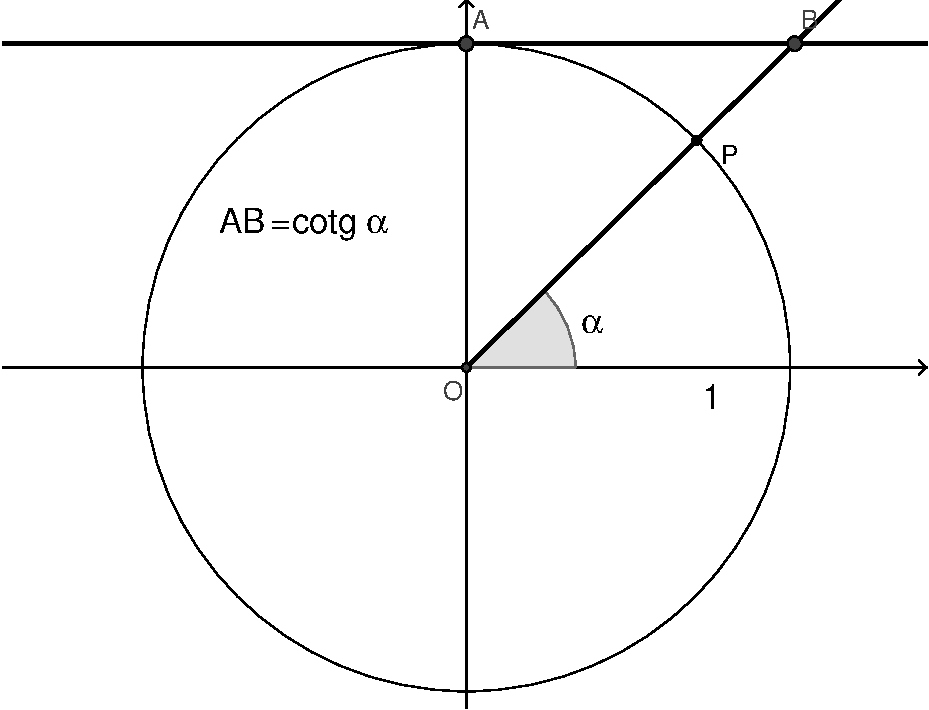
\includegraphics[scale=0.3]{cotgalpha-crop}
		\caption{Cotangente}\label{fig:CotangenteDefinizione}
	\end{subfigure}%
	\begin{subfigure}[b]{.5\linewidth}
		\centering\includegraphics[scale=0.3]{cotgalphagrafico-crop}
		\caption{Cotangente grafico}\label{fig:CotangenteGrafico}
	\end{subfigure}
	\caption{Cotangente}
	\label{tab:funzcotg}
\end{figure}
\begin{definizione}[Cotangente]
	Data una circonferenza goniometrica\nobs\vref{fig:CotangenteDefinizione}, disegno un angolo con centro nell'origine e di ampiezza $\alpha$. Un lato dell'angolo incontra la tangente  alla circonferenza  per $(0;1)$ in un punto $C$.  Chiamo cotangente\index{Funzione!Cotangente!definizione} dell'angolo $\alpha$ e lo indico con $\tg\alpha$ l'ascissa  del punto $C$
\end{definizione}
\subsection{Andamento Cotangente}
\label{sec:AndamentoCotangente}
\begin{table}[tbp]
	\centering
	\renewcommand{\arraystretch}{2}
	\begin{tabular}{rccccc}
	\toprule
	%\backslashbox{Ottengo}{Noto} & $\sen\alpha$ &$\cos\alpha$&$\tg\alpha$ &$\cotg\alpha$ & \multirow{2}{1cm}{$\sen\alpha$ $\cos\alpha$} \\[.5cm]
	& $\sen\alpha$ &$\cos\alpha$&$\tg\alpha$ &$\cotg\alpha$ & $\sen\alpha$, $\cos\alpha$ \\[.6cm]
	\midrule
	$\cos\alpha={}$& $\pm\sqrt{1-\sen^2\alpha}$ & &$\pm\dfrac{1}{\sqrt{1+\tg^2\alpha}}$ & & \\ [.6cm]
	%\hline
	$\sen\alpha={}$& & $\pm\sqrt{1-\cos^2\alpha}$ &$\pm\dfrac{\tg\alpha}{\sqrt{1+\tg^2\alpha}}$ & & \\ [.6cm]
	%\hline
	$\tg\alpha={}$& & & & $\dfrac{1}{\cotg\alpha}$ &$\dfrac{\sen\alpha}{\cos\alpha}$\\ [.6cm]
	%\hline
	$\cotg\alpha={}$& & &$\dfrac{1}{\tg\alpha}$ & &$\dfrac{\cos\alpha}{\sen\alpha}$\\[.6cm] 
	\bottomrule
	\end{tabular}
	\caption{Seno Coseno Tangente Cotangente}
	\label{tab:SenoCosenoTangenteCotangente}
\end{table}
\renewcommand{\arraystretch}{1}
\section{Angoli associati}
\label{sec:goniometriaAngoliAssociati}
\begin{table}[H]
	\centering
	\begin{tikzpicture}[>=triangle 45]
		\draw[->,color=black] (-5.5,0) -- (5.5,0);
	%	\foreach \x in {-5,-4,-3,-2,-1,1,2,3,4,5}
	%	\draw[shift={(\x,0)},color=black] (0pt,-2pt);
		\draw[->,color=black] (0,-5.5) -- (0,5.5);
	%	\foreach \y in {-5,-4,-3,-2,-1,1,2,3,4,5}
		%	\draw[shift={(0,\y)},color=black] (2pt,0pt) -- (-2pt,0pt);
	%	\clip(-5.5,-5.5) rectangle (5.5,5.5);
		%\draw [shift={(0,0)}] (0,0) -- (0:0.96) arc (0:34.65:0.96) -- cycle;
		%\draw [shift={(0,0)}] (0,0) -- (0:1.92) arc (0:145.35:1.92) -- cycle;
		\draw(0,0) circle (5);
		\draw [shift={(0,0)},->] (0:0.96) arc (0:34.65:0.96);
		\draw (4.11,2.84)-- (0,0);
		\draw [dash pattern=on 4pt off 4pt] (-4.11,2.84)-- (4.11,2.84);
		\draw (-4.11,2.84)-- (0,0);
		\draw (5,0)-- (0,0);
		\draw [shift={(0,0)},->] (0:1.92) arc (0:145.35:1.92);
		\draw (0.45,2.45) node[anchor=north west] {$\ang{180}-\alpha$};
		\draw (0.99,0.75) node[anchor=north west] {$\alpha$};
		\draw (-4.11,2.84)-- (-4.11,0);
		\draw (4.11,2.84)-- (4.11,0);
		\draw (-4.04,1.4) node[anchor=north west] {$\sin(\ang{180}-\alpha)$};
		\draw (-2.45,3.56) node[anchor=north west] {$\cos(\ang{180}-\alpha)$};
		\draw (1.98,3.56) node[anchor=north west] {$\cos(\alpha)$};
		\draw (3.31,1.28) node[anchor=north west] {$\sin(\alpha)$};
		\draw (0,0)-- (-4.11,0);
		\fill [color=black] (0,0) circle (1.5pt);
		\draw[color=black] (0.16,0.27) node {$O$};
		\fill [color=black] (4.11,2.84) circle (1.5pt);
		\draw[color=black] (4.26,3.1) node {$C$};
		\fill [color=black] (4.11,2.84) circle (1.5pt);
		%\draw[color=black] (4.26,3.1) node {$D$};
		\fill [color=black] (-4.11,2.84) circle (1.5pt);
		\draw[color=black] (-3.96,3.1) node {$E$};
		\fill [color=black] (-4.11,0) circle (1.5pt);
		\draw[color=black] (-3.98,0.27) node {$F$};
		\fill [color=black] (4.11,0) circle (1.5pt);
		\draw[color=black] (4.26,0.27) node {$G$};
		\fill [color=black] (0,2.84) circle (1.5pt);
		%\draw[color=black] (0.16,3.1) node {$H$};
	\end{tikzpicture}
	\caption{Angoli supplementari $\alpha$ $\ang{180}-\alpha$}
	\label{tab:AngoliAssociatisupplementari}
\end{table}
\begin{table}[H]
	\centering
		\begin{tikzpicture}[line cap=round,line join=round,>=triangle 45,x=1.0cm,y=1.0cm]
			\draw[->,color=black] (-5.5,0) -- (5.5,0);
			%\foreach \x in {-5,-4,-3,-2,-1,1,2,3,4,5}
			%\draw[shift={(\x,0)},color=black] (0pt,-2pt);
			\draw[->,color=black] (0,-5.5) -- (0,5.5);
			%\foreach \y in {-5,-4,-3,-2,-1,1,2,3,4,5}
			%		\draw[shift={(0,\y)},color=black] (2pt,0pt) -- (-2pt,0pt);
		%	\clip(-5.5,-5.5) rectangle (5.5,5.5);
		%	\draw [shift={(0,0)}] (0,0) -- (0:0.85) arc (0:34.65:0.85) -- cycle;
		%	\draw [shift={(0,0)}] (0,0) -- (0:1.7) arc (0:214.65:1.7) -- cycle;
			\draw(0,0) circle (5cm);
			\draw [shift={(0,0)},->] (0:0.85) arc (0:34.65:0.85);
			\draw (4.11,2.84)-- (0,0);
			\draw (5,0)-- (0,0);
			\draw (-2.66,2.04) node[anchor=north west] {$\ang{180}+\alpha$};
			\draw (0.98,0.71) node[anchor=north west] {$\alpha$};
			\draw (4.11,2.84)-- (4.11,0);
			\draw (1.98,3.55) node[anchor=north west] {$\cos(\alpha)$};
			\draw (3.31,1.26) node[anchor=north west] {$\sin(\alpha)$};
			\draw [shift={(0,0)},->] (0:1.7) arc (0:214.65:1.7);
			\draw (0,0)-- (-4.11,-2.84);
			\draw (-4.11,0)-- (-4.11,-2.84);
			\draw [dash pattern=on 4pt off 4pt] (-4.11,-2.84)-- (0,-2.84);
			\draw [dash pattern=on 4pt off 4pt] (0,2.84)-- (4.11,2.84);
			\draw (-4.01,-0.58) node[anchor=north west] {$\sin(\ang{180}+\alpha)$};
			\draw (-2.3,-2.94) node[anchor=north west] {$\cos(\ang{180}+\alpha)$};
			\fill [color=black] (0,0) circle (1.5pt);
			\draw[color=black] (0.13,0.24) node {$O$};
			\fill [color=black] (4.11,2.84) circle (1.5pt);
			\draw[color=black] (4.26,3.07) node {$C$};
			\fill [color=black] (-4.11,0) circle (1.5pt);
			\draw[color=black] (-4,0.24) node {$F$};
			\fill [color=black] (4.11,0) circle (1.5pt);
			\draw[color=black] (4.26,0.24) node {$G$};
			\fill [color=black] (-4.11,-2.84) circle (1.5pt);
			\draw[color=black] (-4,-2.6) node {$J$};
			\fill [color=black] (0,-2.84) circle (1.5pt);
			\draw[color=black] (0.13,-2.6) node {$H$};
			\fill [color=black] (0,2.84) circle (1.5pt);
			\draw[color=black] (0.13,3.07) node {$K$};
		\end{tikzpicture}
			\caption{Angoli che differiscono di $\ang{180}$ $\alpha$ $\ang{180}+\alpha$}
			\label{tab:AngoliAssociatidiff180}
\end{table}
\begin{table}[htbp]
		\centering
			\begin{tikzpicture}[>=triangle 45]
				\draw[->,color=black] (-5.5,0) -- (5.5,0);
				%\foreach \x in {-5,-4,-3,-2,-1,1,2,3,4,5}
				%\draw[shift={(\x,0)},color=black] (0pt,-2pt);
				\draw[->,color=black] (0,-5.5) -- (0,5.5);
				%\foreach \y in {-5,-4,-3,-2,-1,1,2,3,4,5}
				%	\draw[shift={(0,\y)},color=black] (2pt,0pt) -- (-2pt,0pt);
				%\clip(-5.5,-5.5) rectangle (5.5,5.5);
				%\draw [shift={(0,0)}] (0,0) -- (0:0.86) arc (0:34.65:0.86) -- cycle;
				%\draw [shift={(0,0)}] (0,0) -- (0:1.72) arc (0:325.35:1.72) -- cycle;
				\draw(0,0) circle (5);
				\draw [shift={(0,0)},->] (0:0.86) arc (0:34.65:0.86);
				\draw (4.11,2.84)-- (0,0);
				\draw (0.98,0.72) node[anchor=north west] {$\alpha$};
				\draw (1.99,3.55) node[anchor=north west] {$\cos(\alpha)$};
				\draw (3.32,1.26) node[anchor=north west] {$\sin(\alpha)$};
				\draw [shift={(0,0)},->] (0:1.72) arc (0:325.35:1.72);
				\draw (0,0)-- (4.11,-2.84);
				\draw (4.11,2.84)-- (4.11,-2.84);
				\draw [dash pattern=on 4pt off 4pt] (0,2.84)-- (4.11,2.84);
				\draw [dash pattern=on 4pt off 4pt] (0,-2.84)-- (4.11,-2.84);
				\draw (-3,1.1) node[anchor=north west] {$\ang{360}-\alpha$};
				\draw (1.08,-2.82) node[anchor=north west] {$\cos(\ang{360}-\alpha)$};
				\draw (3.3,-0.69) node[anchor=north west] {$\sin(\ang{360}-\alpha)$};
				\fill [color=black] (4.11,2.84) circle (1.5pt);
				%\draw[color=black] (4.25,3.08) node {$C$};
				\fill [color=black] (4.11,2.84) circle (1.5pt);
				\draw[color=black] (4.25,3.08) node {$D$};
				\fill [color=black] (4.11,-2.84) circle (1.5pt);
				\draw[color=black] (4.25,-2.59) node {$E$};
				\fill [color=black] (0,2.84) circle (1.5pt);
				\draw[color=black] (0.14,3.08) node {$H$};
				\fill [color=black] (0,-2.84) circle (1.5pt);
				\draw[color=black] (0.08,-2.59) node {$I$};
			\end{tikzpicture}
			\caption{Angoli esplementari $\alpha$ $\ang{360}-\alpha$}
			\label{tab:AngoliAssociatiopposti}
	\end{table}
\begin{table}[htbp]
	\centering
	\begin{tikzpicture}[>=triangle 45]
		\draw[->,color=black] (-5.5,0) -- (5.5,0);
		%\foreach \x in {-5,-4,-3,-2,-1,1,2,3,4,5}
		%\draw[shift={(\x,0)},color=black] (0pt,-2pt);
		\draw[->,color=black] (0,-5.5) -- (0,5.5);
		%\foreach \y in {-5,-4,-3,-2,-1,1,2,3,4,5}
		%\draw[shift={(0,\y)},color=black] (2pt,0pt) -- (-2pt,0pt);
		%\clip(-5.5,-5.5) rectangle (5.5,5.5);
		%\draw [shift={(0,0)}] (0,0) -- (0:1.72) arc (0:34.65:1.72) -- cycle;
		%\draw [shift={(0,0)}] (0,0) -- (-34.65:1.72) arc (-34.65:0:1.72) -- cycle;
		\draw(0,0) circle (5);
		\draw [shift={(0,0)},->] (0:1.72) arc (0:34.65:1.72);
		\draw (4.11,2.84)-- (0,0);
		\draw (0.98,0.72) node[anchor=north west] {$\alpha$};
		\draw (1.15,3.51) node[anchor=north west] {$\cos(\alpha)$};
		\draw (3.32,1.26) node[anchor=north west] {$\sin(\alpha)$};
		\draw (0,0)-- (4.11,-2.84);
		\draw (4.11,2.84)-- (4.11,-2.84);
		\draw [dash pattern=on 4pt off 4pt] (0,2.84)-- (4.11,2.84);
		\draw [dash pattern=on 4pt off 4pt] (0,-2.84)-- (4.11,-2.84);
		\draw (1.08,-2.82) node[anchor=north west] {$\cos(-\alpha)$};
		\draw (3.3,-0.69) node[anchor=north west] {$\sin(-\alpha)$};
		\draw [shift={(0,0)},-<] (-34.65:1.72) arc (-34.65:0:1.72);
		\draw (0.91,0.09) node[anchor=north west] {$-\alpha$};
		\draw[color=black] (0.14,0.24) node {$O$};
		\draw[color=black] (5.14,0.24) node {$B$};
		%\draw[color=black] (4.25,3.08) node {$C$};
		\draw[color=black] (4.25,3.08) node {$D$};
		\draw[color=black] (4.25,-2.59) node {$E$};
		\draw[color=black] (0.14,3.08) node {$H$};
		\draw[color=black] (0.08,-2.59) node {$I$};
	\end{tikzpicture}
	\caption{Angoli opposti}
	\label{tab:angoliopposti}
\end{table}
\section{Angoli complementari}
\label{sec:angolicomplementari}
\begin{table}[H]
	\centering
	\begin{tikzpicture}[>=triangle 45]
		\draw[->,color=black] (-5.5,0) -- (5.5,0);
		%\foreach \x in {-5,-4,-3,-2,-1,1,2,3,4,5}
		%\draw[shift={(\x,0)},color=black] (0pt,-2pt);
		\draw[->,color=black] (0,-5.5) -- (0,5.5);
		%\foreach \y in {-5,-4,-3,-2,-1,1,2,3,4,5}
		%\draw[shift={(0,\y)},color=black] (2pt,0pt) -- (-2pt,0pt);
		%\clip(-5.5,-5.5) rectangle (5.5,5.5);
		%\draw [shift={(0,0)}] (0,0) -- (0:0.86) arc (0:24.91:0.86) -- cycle;
		%\draw [shift={(0,0)}] (0,0) -- (0:1.72) arc (0:65.09:1.72) -- cycle;
		\draw(0,0) circle (5);
		\draw (0.98,0.72) node[anchor=north west] {$\alpha$};
		\draw (3.32,2.81) node[anchor=north west] {$\cos(\alpha)$};
		\draw (3.66,1.02) node[anchor=north west] {$\sin(\alpha)$};
		\draw (0,0)-- (4.53,2.11);
		\draw [dash pattern=on 4pt off 4pt] (4.53,2.11)-- (4.53,0);
		\draw (0,0)-- (2.11,4.53);
		\draw [shift={(0,0)},->] (0:0.86) arc (0:24.91:0.86);
		\draw [shift={(0,0)},->] (0:1.72) arc (0:65.09:1.72);
		\draw [dash pattern=on 4pt off 4pt] (0,4.53)-- (2.11,4.53);
		\draw [dash pattern=on 1pt off 2pt on 4pt off 4pt] (0,2.11)-- (4.53,2.11);
		\draw [dash pattern=on 1pt off 2pt on 4pt off 4pt] (2.11,4.53)-- (2.11,0);
		\draw (0.34,4.49) node[anchor=north west] {$\cos(\ang{90}-\alpha)$};
		\draw (1.31,1.67) node[anchor=north west] {$\ang{90}-\alpha$};
		\draw (2.23,3.87) node[anchor=north west] {$\sin(\ang{90}-\alpha)$};
		\fill [color=black] (0,0) circle (1.5pt);
		\draw[color=black] (0.14,0.24) node {$O$};
		\fill [color=black] (4.53,2.11) circle (1.5pt);
		\draw[color=black] (4.68,2.34) node {$C$};
		\fill [color=black] (4.53,0) circle (1.5pt);
		\draw[color=black] (4.68,0.24) node {$D$};
		\draw[color=black] (4.3,1.21) node {$d$};
		\fill [color=black] (2.11,4.53) circle (1.5pt);
		\draw[color=black] (2.25,4.78) node {$K$};
		\fill [color=black] (0,4.53) circle (1.5pt);
		\draw[color=black] (0.12,4.78) node {$L$};
		\fill [color=black] (0,2.11) circle (1.5pt);
		\draw[color=black] (0.14,2.34) node {$M$};
		\fill [color=black] (2.11,0) circle (1.5pt);
		\draw[color=black] (2.25,0.24) node {$N$};
	\end{tikzpicture}
		\caption{Angoli complementari $\alpha$ $\ang{90}-\alpha$}
		\label{tab:angolicomplementari1}
\end{table}
\begin{table}
	\centering
	\begin{tikzpicture}[>=triangle 45]
		\draw[->,color=black] (-5.5,0) -- (5.5,0);
		%\foreach \x in {-5,-4,-3,-2,-1,1,2,3,4,5}
		%\draw[shift={(\x,0)},color=black] (0pt,-2pt);
		\draw[->,color=black] (0,-5.5) -- (0,5.5);
		%\foreach \y in {-5,-4,-3,-2,-1,1,2,3,4,5}
		%\draw[shift={(0,\y)},color=black] (2pt,0pt) -- (-2pt,0pt);
		%\clip(-5.5,-5.5) rectangle (5.5,5.5);
		%\draw [shift={(0,0)}] (0,0) -- (0:0.86) arc (0:24.91:0.86) -- cycle;
		%\draw [shift={(0,0)}] (0,0) -- (0:1.72) arc (0:114.91:1.72) -- cycle;
		\draw(0,0) circle (5);
		\draw (0.98,0.72) node[anchor=north west] {$\alpha$};
		\draw (3.32,2.81) node[anchor=north west] {$\cos(\alpha)$};
		\draw (3.66,1.02) node[anchor=north west] {$\sin(\alpha)$};
		\draw (0,0)-- (4.53,2.11);
		\draw [dash pattern=on 4pt off 4pt] (4.53,2.11)-- (4.53,0);
		\draw [shift={(0,0)},->] (0:0.86) arc (0:24.91:0.86);
		\draw [dash pattern=on 1pt off 2pt on 4pt off 4pt] (0,2.11)-- (4.53,2.11);
		\draw (-1.34,4.59) node[anchor=north west] {$\cos(90+\alpha)$};
		\draw (1.31,1.67) node[anchor=north west] {$90+\alpha$};
		\draw (-3.46,2.34) node[anchor=north west] {$\sin(90+\alpha)$};
		\draw (-2.11,4.53)-- (0,0);
		\draw [dash pattern=on 4pt off 4pt] (-2.11,4.53)-- (0,4.53);
		\draw [dash pattern=on 1pt off 2pt on 4pt off 4pt] (-2.11,4.53)-- (-2.11,0);
		\draw [shift={(0,0)},->] (0:1.72) arc (0:114.91:1.72);
		\fill [color=black] (0,0) circle (1.5pt);
		\draw[color=black] (0.14,0.24) node {$O$};
		\fill [color=black] (4.53,2.11) circle (1.5pt);
		\draw[color=black] (4.68,2.34) node {$C$};
		\fill [color=black] (4.53,0) circle (1.5pt);
		\draw[color=black] (4.68,0.24) node {$D$};
		\fill [color=black] (-2.11,0) circle (1.5pt);
		\draw[color=black] (-1.96,0.24) node {$H$};
		\fill [color=black] (0,2.11) circle (1.5pt);
		\draw[color=black] (0.14,2.34) node {$M$};
		\fill [color=black] (-2.11,4.53) circle (1.5pt);
		\draw[color=black] (-1.96,4.78) node {$K$};
		\fill [color=black] (0,4.53) circle (1.5pt);
		\draw[color=black] (0.12,4.78) node {$L$};
	\end{tikzpicture}
\caption{Angoli complementari $\alpha$ $\ang{90}+\alpha$}
\label{tab:angolicomplementari2}
\end{table}
\begin{table}[H]
	\centering
		\begin{tikzpicture}[>=triangle 45]
			\draw[->,color=black] (-5.5,0) -- (5.5,0);
			%\foreach \x in {-5,-4,-3,-2,-1,1,2,3,4,5}
			%\draw[shift={(\x,0)},color=black] (0pt,-2pt);
			\draw[->,color=black] (0,-5.5) -- (0,5.5);
			%\foreach \y in {-5,-4,-3,-2,-1,1,2,3,4,5}
			%\draw[shift={(0,\y)},color=black] (2pt,0pt) -- (-2pt,0pt);
			%\clip(-5.5,-5.5) rectangle (5.5,5.5);
			%\draw [shift={(0,0)}] (0,0) -- (0:0.86) arc (0:24.91:0.86) -- cycle;
			%\draw [shift={(0,0)}] (0,0) -- (0:1.72) arc (0:245.09:1.72) -- cycle;
			\draw(0,0) circle (5);
			\draw (0.98,0.72) node[anchor=north west] {$\alpha$};
			\draw (3.32,2.81) node[anchor=north west] {$\cos(\alpha)$};
			\draw (3.66,1.02) node[anchor=north west] {$\sin(\alpha)$};
			\draw (0,0)-- (4.53,2.11);
			\draw [dash pattern=on 4pt off 4pt] (4.53,2.11)-- (4.53,0);
			\draw [shift={(0,0)},->] (0:0.86) arc (0:24.91:0.86);
			\draw [dash pattern=on 1pt off 2pt on 4pt off 4pt] (0,2.11)-- (4.53,2.11);
			\draw (-1.43,-3.52) node[anchor=north west] {$\cos(270-\alpha)$};
			\draw (-1.64,2.08) node[anchor=north west] {$270-\alpha$};
			\draw (-3.7,-1.97) node[anchor=north west] {$\sin(270-\alpha)$};
			\draw [dash pattern=on 1pt off 2pt on 4pt off 4pt] (-2.11,0)-- (-2.11,-4.53);
			\draw (0,0)-- (-2.11,-4.53);
			\draw [shift={(0,0)},->] (0:1.72) arc (0:245.09:1.72);
			\draw [dash pattern=on 4pt off 4pt] (-2.11,-4.53)-- (0,-4.53);
			\fill [color=black] (0,0) circle (1.5pt);
			\draw[color=black] (0.14,0.24) node {$O$};
			\fill [color=black] (4.53,2.11) circle (1.5pt);
			\draw[color=black] (4.68,2.34) node {$C$};
			\fill [color=black] (4.53,0) circle (1.5pt);
			\draw[color=black] (4.68,0.24) node {$D$};
			\fill [color=black] (-2.11,0) circle (1.5pt);
			\draw[color=black] (-1.96,0.24) node {$H$};
			\fill [color=black] (0,2.11) circle (1.5pt);
			\draw[color=black] (0.14,2.34) node {$M$};
			\fill [color=black] (-2.11,-4.53) circle (1.5pt);
			\draw[color=black] (-1.98,-4.3) node {$J$};
			\fill [color=black] (0,-4.53) circle (1.5pt);
			\draw[color=black] (0.12,-4.3) node {$L$};
		\end{tikzpicture}
		\caption{Angoli complementari $\alpha$ $\ang{270}-\alpha$}
		\label{tab:angolicomplementari3}
\end{table}
\mediapriorita{Manca la tabella 270+$\alpha$}
\begin{table}
	\footnotesize
	\centering
	\begin{tabular}{rlllllll}
	\toprule
	$\sen\alpha=$&$\cos(\ang{90}-\alpha)$&$-\cos(\ang{90}+\alpha)$&$\sen(\ang{180}-\alpha)$&$-\sen(\ang{180}+\alpha)$&$-\cos(\ang{270}-\alpha)$&$\cos(\ang{270}+\alpha)$&$-\sen(-\alpha)$\\[.6cm] 
	$\cos\alpha=$&$\sen(\ang{90}-\alpha)$&$\sen(\ang{90}+\alpha)$&$-\cos(\ang{180}-\alpha)$&$-\cos(\ang{180}+\alpha)$&$-\sen(\ang{270}-\alpha)$&$-\sen(\ang{270}+\alpha)$&$\cos(-\alpha)$\\[.6cm] 
	$\tg\alpha=$&$\cotg(\ang{90}-\alpha)$&$-\cotg(\ang{90}+\alpha)$&$-\tg(\ang{180}-\alpha)$&$\tg(\ang{180}+\alpha)$&$\cotg(\ang{270}-\alpha)$&$-\cotg(\ang{270}+\alpha)$&$-\tg(-\alpha)$\\[.6cm] 
	$\cotg\alpha=$&$\tg(\ang{90}-\alpha)$&$-\tg(\ang{90}+\alpha)$&$-\cotg(\ang{180}-\alpha)$&$\cotg(\ang{180}+\alpha)$&$\tg(\ang{270}-\alpha)$&$-\tg(\ang{270}+\alpha)$&$-\cotg(-\alpha)$\\[.6cm]
	\bottomrule
	\end{tabular}
	\caption{Angoli complementari e supplementari}
	\label{tab:differnzediangoli}
\end{table}
\section{Formule di addizione e sottrazione}
\label{sec:Formulediaddizionesottrazione}
\subsection{Coseno della differenza di due angoli}
\label{sec:cosenodifferenza}

\begin{table}[H]
	\centering
	\begin{tikzpicture}[>=triangle 45]
		\draw[->,color=black] (-5.5,0) -- (5.5,0);
		%\foreach \x in {-4,-2,2,4}
		%\draw[shift={(\x,0)},color=black] (0pt,-2pt);
		\draw[->,color=black] (0,-5.5) -- (0,5.5);
		%\foreach \y in {-4,-2,2,4}
		%	\draw[shift={(0,\y)},color=black] (2pt,0pt) -- (-2pt,0pt);
		%\clip(-5.5,-5.5) rectangle (5.5,5.5);
%		\draw [shift={(0,0)}] (0,0) -- (0:2.29) arc (0:214:2.29) -- cycle;
%		\draw [shift={(0,0)}] (0,0) -- (0:1.14) arc (0:166.13:1.14) -- cycle;
%		\draw [shift={(0,0)}] (0,0) -- (166.13:1.6) arc (166.13:214:1.6) -- cycle;
%		\draw [shift={(0,0)}] (0,0) -- (0:1.6) arc (0:47.87:1.6) -- cycle;
		\draw(0,0) circle (5);
		\draw (0,0)-- (-4.15,-2.8);
		\draw [shift={(0,0)},->] (0:2.29) arc (0:214:2.29);
		\draw (0,0)-- (-4.85,1.2);
		\draw [shift={(0,0)},->] (0:1.14) arc (0:166.13:1.14);
		\draw [shift={(0,0)}] (166.13:1.6) arc (166.13:214:1.6);
		\draw(-1.48,-0.39) -- (-1.62,-0.43);
		\draw(-1.53,-0.14) -- (-1.66,-0.15);
		\draw (-4.85,1.2)-- (-4.15,-2.8);
		\draw [shift={(0,0)}] (0:1.6) arc (0:47.87:1.6);
		\draw(1.34,0.74) -- (1.47,0.8);
		\draw(1.45,0.5) -- (1.58,0.55);
		\draw (3.35,3.71)-- (5,0);
		\draw (3.35,3.71)-- (0,0);
		\draw (-2.06,2.1) node[anchor=north west] {$\alpha$};
		\draw (-1.03,1.46) node[anchor=north west] {$\beta$};
		\draw (-4.05,-0.62) node[anchor=north west] {$\alpha - \beta$};
		\draw (2.38,1.74) node[anchor=north west] {$\alpha-\beta$};
		\fill [color=black] (0,0) circle (1.5pt);
		\draw[color=black] (0.19,0.32) node {$O$};
		\fill [color=black] (5,0) circle (1.5pt);
		\draw[color=black] (5.18,0.32) node {$D$};
		\fill [color=black] (-4.15,-2.8) circle (1.5pt);
		\draw[color=black] (-3.98,-2.47) node {$A$};
		\fill [color=black] (-4.85,1.2) circle (1.5pt);
		\draw[color=black] (-4.66,1.51) node {$B$};
		\fill [color=black] (3.35,3.71) circle (1.5pt);
		\draw[color=black] (3.53,4.03) node {$C$};
	\end{tikzpicture}
	\caption{Differenza di angoli}
\end{table}
\begin{table}[H]
	\centering
	$
	\begin{array}{cc}
	\toprule
	\cos(\alpha-\beta)=	&\cos\alpha\cos\beta+\sen\alpha\sen\beta \\ 
	\cos(\alpha+\beta)=	&\cos\alpha\cos\beta-\sen\alpha\sen\beta \\ 
	\sen\left(\alpha-\beta\right)={} &\sen\alpha\cos\beta-\cos\alpha\sen\beta\\
\sen\left(\alpha+\beta\right)={}&\sen\alpha\cos\beta+\cos\alpha\sen\beta\\
	\bottomrule
	\end{array}
	$ 
	\caption{ Seno e Coseno, somma o differenza di angoli}
	\label{Tab:sommadifferenzacosenoseno}
\end{table}
\section{Funzioni Sinusoidali}
\label{sec:FunzioniSinusoidali}
\begin{figure}[H]
	\begin{subfigure}[b]{.5\linewidth}
		\centering% Tikz File 'mytikz.tex'
\documentclass{standalone}
%\input{../../Mod_base/grafica}
\input{../Mod_base/grafica}
%italianizziomo gli operatori

\DeclareMathOperator{\sen}{sen}
\DeclareMathOperator{\tg}{tg}
\DeclareMathOperator{\cotg}{cotg}
\DeclareMathOperator{\arcsen}{arcsen}
\DeclareMathOperator{\arctg}{arctg}
\DeclareMathOperator{\arccotg}{arccotg}
%\DeclareMathOperator{\sec}{sec}
\DeclareMathOperator{\cosec}{cosec}
\providecommand{\abs}[1]{\lvert#1\rvert}
\providecommand{\norm}[1]{\lVert#1\rVert} 
%\newcommand{\gradi}{\ensuremath{^\circ}}
%\newcommand{\gradi}{\ensuremath{\degree}}
%\newcommand{\minuti}{\ensuremath{\arcminute}}
\newcommand{\PA}[1]{\boldsymbol{\mathcal{#1}}}
\newcommand{\PDA}{\PA{P}}
\newcommand{\numberset}[1]{\boldsymbol{\mathbb{#1}}}
\newcommand{\N}{\numberset{N}}
\newcommand{\Nz}{\numberset{N}^{}_{0}}
\newcommand{\Z}{\numberset{Z}}
\newcommand{\Zn}{\numberset{Z^{-}}}
\newcommand{\Zp}{\numberset{Z^{+}}}
\newcommand{\Q}{\numberset{Q}}
\newcommand{\Qp}{\numberset{Q^{+}}}
\newcommand{\Qn}{\numberset{Q^{-}}}
\newcommand{\R}{\numberset{R}}
\newcommand{\Rp}{\numberset{R^{+}}}
\newcommand{\Rn}{\numberset{R^{-}}}
\newcommand{\nq}{\ensuremath{\mathbb{Q}}}
\newcommand{\bld}[1]{\mbox{\boldmath $#1$}}
\newcommand{\C}{\numberset{C}}
%spazi fantasma
%\newcommand{\spa}{\phantom{1}}
%\let\origcleardoublepage\cleardoublepage
%\newcommand{\clearemptydoublepage}{%
%\clearpage
%{\pagestyle{empty}\origcleardoublepage}%
%}
%\let\cleardoublepage\clearemptydoublepage
%spazio insecabile
%\newcommand{\nbs}{\nobreakspace}
%le costanti
\newcommand{\costante}{\textrm{costante}}
\DeclareMathOperator{\uimm}{j}
  \let\Re\undefined\DeclareMathOperator{\Re}{Re}
  \let\Im\undefined\DeclareMathOperator{\Im}{Im}
\DeclareMathOperator{\mcd}{mcd}
\DeclareMathOperator{\mcm}{mcm}
\input{../Mod_base/unita_misura}
%\usetikzlibrary{...}
\begin{document}
	
		\begin{tikzpicture}[>=triangle 45]
		\draw[->,color=black] (-0.5,0) -- (7,0);
		%\foreach \x in {,1,2,3,4,5,6,7}
		%\draw[shift={(\x,0)},color=black] (0pt,-2pt);
		\draw[color=black] (6.83,0.09) node [anchor=south west] { t};
		\draw[->,color=black] (0,-6) -- (0,6);
		%\foreach \y in {-6,-4,-2,2,4,6}
		%\draw[shift={(0,\y)},color=black] (-2pt,0pt);
		\draw[color=black] (0.06,5.55) node [anchor=west] { y};
		%\clip(-0.5,-6) rectangle (7,6);
		\draw plot[raw gnuplot, id=func0] function{set samples 100; set xrange [0.0:6.28]; plot 5*sin(x)};
		\draw (4.11,2.79) node[anchor=north west] {$y=A\sin\omega t$};
		\draw [dash pattern=on 6pt off 6pt] (1.57,5)-- (1.57,0);
		\draw [dash pattern=on 6pt off 6pt] (4.71,0)-- (4.71,-5);
		\draw (-0.13,-0.25) node[anchor=north west] {\textbf{0}};
		\draw (1.47,0.08) node[anchor=north west] {$\mathbf{\dfrac{T}{4}}$};
		\draw (3.05,0.08) node[anchor=north west] {$\mathbf{\dfrac{T}{2}}$};
		\draw (4.55,0.08) node[anchor=north west] {$\mathbf{\dfrac{3}{4}T}$};
		\draw (6.25,0.08) node[anchor=north west] {$\mathbf{T}$};
		\draw (0,5)-- (1.57,5);
		\draw (0,-5)-- (4.71,-5);
		\draw (0.51,5.17) node[anchor=north west] {$\mathbf{A}$};
		\draw (1.17,-4.14) node[anchor=north west] {$\mathbf{-A}$};
		\fill [color=black] (1.57,0) circle (1.5pt);
		\fill [color=black] (1.57,5) circle (1.5pt);
		\fill [color=black] (4.71,0) circle (1.5pt);
		\fill [color=black] (4.71,-5) circle (1.5pt);
		\fill [color=black] (3.14,0) circle (1.5pt);
		\fill [color=black] (6.28,0) circle (1.5pt);
		\fill [color=black] (0,5) circle (1.5pt);
		\fill [color=black] (0,-5) circle (1.5pt);
		\end{tikzpicture}
\end{document}
		\caption{Grafico di $y=A\sen\omega t$}\label{fig:asinomegat}
	\end{subfigure}%
	\qquad\qquad
	\begin{subfigure}[b]{.5\linewidth}
		\centering% Tikz File 'mytikz.tex'
\documentclass{standalone}
%\input{../../Mod_base/grafica}
\input{../Mod_base/grafica}
%italianizziomo gli operatori

\DeclareMathOperator{\sen}{sen}
\DeclareMathOperator{\tg}{tg}
\DeclareMathOperator{\cotg}{cotg}
\DeclareMathOperator{\arcsen}{arcsen}
\DeclareMathOperator{\arctg}{arctg}
\DeclareMathOperator{\arccotg}{arccotg}
%\DeclareMathOperator{\sec}{sec}
\DeclareMathOperator{\cosec}{cosec}
\providecommand{\abs}[1]{\lvert#1\rvert}
\providecommand{\norm}[1]{\lVert#1\rVert} 
%\newcommand{\gradi}{\ensuremath{^\circ}}
%\newcommand{\gradi}{\ensuremath{\degree}}
%\newcommand{\minuti}{\ensuremath{\arcminute}}
\newcommand{\PA}[1]{\boldsymbol{\mathcal{#1}}}
\newcommand{\PDA}{\PA{P}}
\newcommand{\numberset}[1]{\boldsymbol{\mathbb{#1}}}
\newcommand{\N}{\numberset{N}}
\newcommand{\Nz}{\numberset{N}^{}_{0}}
\newcommand{\Z}{\numberset{Z}}
\newcommand{\Zn}{\numberset{Z^{-}}}
\newcommand{\Zp}{\numberset{Z^{+}}}
\newcommand{\Q}{\numberset{Q}}
\newcommand{\Qp}{\numberset{Q^{+}}}
\newcommand{\Qn}{\numberset{Q^{-}}}
\newcommand{\R}{\numberset{R}}
\newcommand{\Rp}{\numberset{R^{+}}}
\newcommand{\Rn}{\numberset{R^{-}}}
\newcommand{\nq}{\ensuremath{\mathbb{Q}}}
\newcommand{\bld}[1]{\mbox{\boldmath $#1$}}
\newcommand{\C}{\numberset{C}}
%spazi fantasma
%\newcommand{\spa}{\phantom{1}}
%\let\origcleardoublepage\cleardoublepage
%\newcommand{\clearemptydoublepage}{%
%\clearpage
%{\pagestyle{empty}\origcleardoublepage}%
%}
%\let\cleardoublepage\clearemptydoublepage
%spazio insecabile
%\newcommand{\nbs}{\nobreakspace}
%le costanti
\newcommand{\costante}{\textrm{costante}}
\DeclareMathOperator{\uimm}{j}
  \let\Re\undefined\DeclareMathOperator{\Re}{Re}
  \let\Im\undefined\DeclareMathOperator{\Im}{Im}
\DeclareMathOperator{\mcd}{mcd}
\DeclareMathOperator{\mcm}{mcm}
\input{../Mod_base/unita_misura}
%\usetikzlibrary{...}
\begin{document}
	
\begin{tikzpicture}[>=triangle 45]
\draw[->,color=black] (-0.5,0) -- (7,0);
%\foreach \x in {,1,2,3,4,5,6,7}
%\draw[shift={(\x,0)},color=black] (0pt,-2pt);
\draw[color=black] (6.85,0.09) node [anchor=south west] { t};
\draw[->,color=black] (0,-6) -- (0,6);
%\foreach \y in {-6,-4,-2,2,4,6}
%\draw[shift={(0,\y)},color=black] (-2pt,0pt);
\draw[color=black] (0.06,5.5) node [anchor=west] { y};
%\clip(-0.5,-6) rectangle (7,6);
\draw (2.45,2.58) node[anchor=north west] {$y=A\cos\omega t$};
\draw [dash pattern=on 6pt off 6pt] (3.14,0)-- (3.14,-5);
\draw (-0.13,-0.08) node[anchor=north west] {\textbf{0}};
\draw (1.47,0.08) node[anchor=north west] {$\mathbf{\dfrac{T}{4}}$};
\draw plot[raw gnuplot, id=func0] function{set samples 100; set xrange [0.0:6.28]; plot 5*cos(x)};
\draw (3.05,0.08) node[anchor=north west] {$\mathbf{\dfrac{T}{2}}$};
\draw (4.55,0.08) node[anchor=north west] {$\mathbf{\dfrac{3}{4}T}$};
\draw (6.25,0.08) node[anchor=north west] {$\mathbf{T}$};
\draw (0,-5)-- (3.14,-5);
\draw (0.51,5.2) node[anchor=north west] {$\mathbf{A}$};
\draw (0.49,-4.04) node[anchor=north west] {$\mathbf{-A}$};
\draw [dash pattern=on 6pt off 6pt] (6.28,5)-- (6.28,0);
\fill [color=black] (1.57,0) circle (1.5pt);
\fill [color=black] (3.14,0) circle (1.5pt);
\fill [color=black] (3.14,-5) circle (1.5pt);
\fill [color=black] (0,5) circle (1.5pt);
\fill [color=black] (0,-5) circle (1.5pt);
\fill [color=black] (6.28,0) circle (1.5pt);
\fill [color=black] (6.28,0) circle (1.5pt);
\fill [color=black] (6.28,5) circle (1.5pt);
\end{tikzpicture}
\end{document}
		\caption{Grafico di $y=A\cos\omega t$}\label{fig:acosomegat}
	\end{subfigure}
	\caption{Funzioni sinusoidali}
	\label{fig:Funzionisinusoidali}
\end{figure}
%\begin{table}[H]
%\centering
%%\subfloat[][Grafico di $y=A\sen\omega t$\label{fig:asinomegat}]
%{% Tikz File 'mytikz.tex'
\documentclass{standalone}
%\input{../../Mod_base/grafica}
\input{../Mod_base/grafica}
%italianizziomo gli operatori

\DeclareMathOperator{\sen}{sen}
\DeclareMathOperator{\tg}{tg}
\DeclareMathOperator{\cotg}{cotg}
\DeclareMathOperator{\arcsen}{arcsen}
\DeclareMathOperator{\arctg}{arctg}
\DeclareMathOperator{\arccotg}{arccotg}
%\DeclareMathOperator{\sec}{sec}
\DeclareMathOperator{\cosec}{cosec}
\providecommand{\abs}[1]{\lvert#1\rvert}
\providecommand{\norm}[1]{\lVert#1\rVert} 
%\newcommand{\gradi}{\ensuremath{^\circ}}
%\newcommand{\gradi}{\ensuremath{\degree}}
%\newcommand{\minuti}{\ensuremath{\arcminute}}
\newcommand{\PA}[1]{\boldsymbol{\mathcal{#1}}}
\newcommand{\PDA}{\PA{P}}
\newcommand{\numberset}[1]{\boldsymbol{\mathbb{#1}}}
\newcommand{\N}{\numberset{N}}
\newcommand{\Nz}{\numberset{N}^{}_{0}}
\newcommand{\Z}{\numberset{Z}}
\newcommand{\Zn}{\numberset{Z^{-}}}
\newcommand{\Zp}{\numberset{Z^{+}}}
\newcommand{\Q}{\numberset{Q}}
\newcommand{\Qp}{\numberset{Q^{+}}}
\newcommand{\Qn}{\numberset{Q^{-}}}
\newcommand{\R}{\numberset{R}}
\newcommand{\Rp}{\numberset{R^{+}}}
\newcommand{\Rn}{\numberset{R^{-}}}
\newcommand{\nq}{\ensuremath{\mathbb{Q}}}
\newcommand{\bld}[1]{\mbox{\boldmath $#1$}}
\newcommand{\C}{\numberset{C}}
%spazi fantasma
%\newcommand{\spa}{\phantom{1}}
%\let\origcleardoublepage\cleardoublepage
%\newcommand{\clearemptydoublepage}{%
%\clearpage
%{\pagestyle{empty}\origcleardoublepage}%
%}
%\let\cleardoublepage\clearemptydoublepage
%spazio insecabile
%\newcommand{\nbs}{\nobreakspace}
%le costanti
\newcommand{\costante}{\textrm{costante}}
\DeclareMathOperator{\uimm}{j}
  \let\Re\undefined\DeclareMathOperator{\Re}{Re}
  \let\Im\undefined\DeclareMathOperator{\Im}{Im}
\DeclareMathOperator{\mcd}{mcd}
\DeclareMathOperator{\mcm}{mcm}
\input{../Mod_base/unita_misura}
%\usetikzlibrary{...}
\begin{document}
	
		\begin{tikzpicture}[>=triangle 45]
		\draw[->,color=black] (-0.5,0) -- (7,0);
		%\foreach \x in {,1,2,3,4,5,6,7}
		%\draw[shift={(\x,0)},color=black] (0pt,-2pt);
		\draw[color=black] (6.83,0.09) node [anchor=south west] { t};
		\draw[->,color=black] (0,-6) -- (0,6);
		%\foreach \y in {-6,-4,-2,2,4,6}
		%\draw[shift={(0,\y)},color=black] (-2pt,0pt);
		\draw[color=black] (0.06,5.55) node [anchor=west] { y};
		%\clip(-0.5,-6) rectangle (7,6);
		\draw plot[raw gnuplot, id=func0] function{set samples 100; set xrange [0.0:6.28]; plot 5*sin(x)};
		\draw (4.11,2.79) node[anchor=north west] {$y=A\sin\omega t$};
		\draw [dash pattern=on 6pt off 6pt] (1.57,5)-- (1.57,0);
		\draw [dash pattern=on 6pt off 6pt] (4.71,0)-- (4.71,-5);
		\draw (-0.13,-0.25) node[anchor=north west] {\textbf{0}};
		\draw (1.47,0.08) node[anchor=north west] {$\mathbf{\dfrac{T}{4}}$};
		\draw (3.05,0.08) node[anchor=north west] {$\mathbf{\dfrac{T}{2}}$};
		\draw (4.55,0.08) node[anchor=north west] {$\mathbf{\dfrac{3}{4}T}$};
		\draw (6.25,0.08) node[anchor=north west] {$\mathbf{T}$};
		\draw (0,5)-- (1.57,5);
		\draw (0,-5)-- (4.71,-5);
		\draw (0.51,5.17) node[anchor=north west] {$\mathbf{A}$};
		\draw (1.17,-4.14) node[anchor=north west] {$\mathbf{-A}$};
		\fill [color=black] (1.57,0) circle (1.5pt);
		\fill [color=black] (1.57,5) circle (1.5pt);
		\fill [color=black] (4.71,0) circle (1.5pt);
		\fill [color=black] (4.71,-5) circle (1.5pt);
		\fill [color=black] (3.14,0) circle (1.5pt);
		\fill [color=black] (6.28,0) circle (1.5pt);
		\fill [color=black] (0,5) circle (1.5pt);
		\fill [color=black] (0,-5) circle (1.5pt);
		\end{tikzpicture}
\end{document}}
%\subfloat[][Grafico di $y=A\cos\omega t$\label{fig:acosomegat}]{
%% Tikz File 'mytikz.tex'
\documentclass{standalone}
%\input{../../Mod_base/grafica}
\input{../Mod_base/grafica}
%italianizziomo gli operatori

\DeclareMathOperator{\sen}{sen}
\DeclareMathOperator{\tg}{tg}
\DeclareMathOperator{\cotg}{cotg}
\DeclareMathOperator{\arcsen}{arcsen}
\DeclareMathOperator{\arctg}{arctg}
\DeclareMathOperator{\arccotg}{arccotg}
%\DeclareMathOperator{\sec}{sec}
\DeclareMathOperator{\cosec}{cosec}
\providecommand{\abs}[1]{\lvert#1\rvert}
\providecommand{\norm}[1]{\lVert#1\rVert} 
%\newcommand{\gradi}{\ensuremath{^\circ}}
%\newcommand{\gradi}{\ensuremath{\degree}}
%\newcommand{\minuti}{\ensuremath{\arcminute}}
\newcommand{\PA}[1]{\boldsymbol{\mathcal{#1}}}
\newcommand{\PDA}{\PA{P}}
\newcommand{\numberset}[1]{\boldsymbol{\mathbb{#1}}}
\newcommand{\N}{\numberset{N}}
\newcommand{\Nz}{\numberset{N}^{}_{0}}
\newcommand{\Z}{\numberset{Z}}
\newcommand{\Zn}{\numberset{Z^{-}}}
\newcommand{\Zp}{\numberset{Z^{+}}}
\newcommand{\Q}{\numberset{Q}}
\newcommand{\Qp}{\numberset{Q^{+}}}
\newcommand{\Qn}{\numberset{Q^{-}}}
\newcommand{\R}{\numberset{R}}
\newcommand{\Rp}{\numberset{R^{+}}}
\newcommand{\Rn}{\numberset{R^{-}}}
\newcommand{\nq}{\ensuremath{\mathbb{Q}}}
\newcommand{\bld}[1]{\mbox{\boldmath $#1$}}
\newcommand{\C}{\numberset{C}}
%spazi fantasma
%\newcommand{\spa}{\phantom{1}}
%\let\origcleardoublepage\cleardoublepage
%\newcommand{\clearemptydoublepage}{%
%\clearpage
%{\pagestyle{empty}\origcleardoublepage}%
%}
%\let\cleardoublepage\clearemptydoublepage
%spazio insecabile
%\newcommand{\nbs}{\nobreakspace}
%le costanti
\newcommand{\costante}{\textrm{costante}}
\DeclareMathOperator{\uimm}{j}
  \let\Re\undefined\DeclareMathOperator{\Re}{Re}
  \let\Im\undefined\DeclareMathOperator{\Im}{Im}
\DeclareMathOperator{\mcd}{mcd}
\DeclareMathOperator{\mcm}{mcm}
\input{../Mod_base/unita_misura}
%\usetikzlibrary{...}
\begin{document}
	
\begin{tikzpicture}[>=triangle 45]
\draw[->,color=black] (-0.5,0) -- (7,0);
%\foreach \x in {,1,2,3,4,5,6,7}
%\draw[shift={(\x,0)},color=black] (0pt,-2pt);
\draw[color=black] (6.85,0.09) node [anchor=south west] { t};
\draw[->,color=black] (0,-6) -- (0,6);
%\foreach \y in {-6,-4,-2,2,4,6}
%\draw[shift={(0,\y)},color=black] (-2pt,0pt);
\draw[color=black] (0.06,5.5) node [anchor=west] { y};
%\clip(-0.5,-6) rectangle (7,6);
\draw (2.45,2.58) node[anchor=north west] {$y=A\cos\omega t$};
\draw [dash pattern=on 6pt off 6pt] (3.14,0)-- (3.14,-5);
\draw (-0.13,-0.08) node[anchor=north west] {\textbf{0}};
\draw (1.47,0.08) node[anchor=north west] {$\mathbf{\dfrac{T}{4}}$};
\draw plot[raw gnuplot, id=func0] function{set samples 100; set xrange [0.0:6.28]; plot 5*cos(x)};
\draw (3.05,0.08) node[anchor=north west] {$\mathbf{\dfrac{T}{2}}$};
\draw (4.55,0.08) node[anchor=north west] {$\mathbf{\dfrac{3}{4}T}$};
\draw (6.25,0.08) node[anchor=north west] {$\mathbf{T}$};
\draw (0,-5)-- (3.14,-5);
\draw (0.51,5.2) node[anchor=north west] {$\mathbf{A}$};
\draw (0.49,-4.04) node[anchor=north west] {$\mathbf{-A}$};
\draw [dash pattern=on 6pt off 6pt] (6.28,5)-- (6.28,0);
\fill [color=black] (1.57,0) circle (1.5pt);
\fill [color=black] (3.14,0) circle (1.5pt);
\fill [color=black] (3.14,-5) circle (1.5pt);
\fill [color=black] (0,5) circle (1.5pt);
\fill [color=black] (0,-5) circle (1.5pt);
\fill [color=black] (6.28,0) circle (1.5pt);
\fill [color=black] (6.28,0) circle (1.5pt);
\fill [color=black] (6.28,5) circle (1.5pt);
\end{tikzpicture}
\end{document}}
%\caption{Funzioni sinusoidali}
%\label{fig:Funzionisinusoidali}
%\end{table}
\begin{figure}[H]
	\begin{subfigure}[b]{.5\linewidth}
		\centering% Tikz File 'mytikz.tex'
\documentclass{standalone}
%\input{../../Mod_base/grafica}
\input{../Mod_base/grafica}
%italianizziomo gli operatori

\DeclareMathOperator{\sen}{sen}
\DeclareMathOperator{\tg}{tg}
\DeclareMathOperator{\cotg}{cotg}
\DeclareMathOperator{\arcsen}{arcsen}
\DeclareMathOperator{\arctg}{arctg}
\DeclareMathOperator{\arccotg}{arccotg}
%\DeclareMathOperator{\sec}{sec}
\DeclareMathOperator{\cosec}{cosec}
\providecommand{\abs}[1]{\lvert#1\rvert}
\providecommand{\norm}[1]{\lVert#1\rVert} 
%\newcommand{\gradi}{\ensuremath{^\circ}}
%\newcommand{\gradi}{\ensuremath{\degree}}
%\newcommand{\minuti}{\ensuremath{\arcminute}}
\newcommand{\PA}[1]{\boldsymbol{\mathcal{#1}}}
\newcommand{\PDA}{\PA{P}}
\newcommand{\numberset}[1]{\boldsymbol{\mathbb{#1}}}
\newcommand{\N}{\numberset{N}}
\newcommand{\Nz}{\numberset{N}^{}_{0}}
\newcommand{\Z}{\numberset{Z}}
\newcommand{\Zn}{\numberset{Z^{-}}}
\newcommand{\Zp}{\numberset{Z^{+}}}
\newcommand{\Q}{\numberset{Q}}
\newcommand{\Qp}{\numberset{Q^{+}}}
\newcommand{\Qn}{\numberset{Q^{-}}}
\newcommand{\R}{\numberset{R}}
\newcommand{\Rp}{\numberset{R^{+}}}
\newcommand{\Rn}{\numberset{R^{-}}}
\newcommand{\nq}{\ensuremath{\mathbb{Q}}}
\newcommand{\bld}[1]{\mbox{\boldmath $#1$}}
\newcommand{\C}{\numberset{C}}
%spazi fantasma
%\newcommand{\spa}{\phantom{1}}
%\let\origcleardoublepage\cleardoublepage
%\newcommand{\clearemptydoublepage}{%
%\clearpage
%{\pagestyle{empty}\origcleardoublepage}%
%}
%\let\cleardoublepage\clearemptydoublepage
%spazio insecabile
%\newcommand{\nbs}{\nobreakspace}
%le costanti
\newcommand{\costante}{\textrm{costante}}
\DeclareMathOperator{\uimm}{j}
  \let\Re\undefined\DeclareMathOperator{\Re}{Re}
  \let\Im\undefined\DeclareMathOperator{\Im}{Im}
\DeclareMathOperator{\mcd}{mcd}
\DeclareMathOperator{\mcm}{mcm}
\input{../Mod_base/unita_misura}
%\usetikzlibrary{...}
\begin{document}
	
\begin{tikzpicture}[>=triangle 45]
\draw[->,color=black] (-0.5,0) -- (7,0);
%\foreach \x in {,1,2,3,4,5,6,7}
%\draw[shift={(\x,0)},color=black] (0pt,-2pt);
\draw[color=black] (6.85,0.09) node [anchor=south west] { t};
\draw[->,color=black] (0,-6) -- (0,6);
%\foreach \y in {-6,-4,-2,2,4,6}
%\draw[shift={(0,\y)},color=black] (-2pt,0pt);
\draw[color=black] (0.06,5.5) node [anchor=west] { y};
%\clip(-0.5,-6) rectangle (7,6);
\draw (4.3,4.4) node[anchor=north west] {$\mathbf{y=A\sin\omega_{1} t}$};
\draw [dash pattern=on 6pt off 6pt] (1.57,5)-- (1.57,0);
\draw (-0.13,0.08) node[anchor=north west] {\textbf{0}};
\draw (1.47,0.08) node[anchor=north west] {$\mathbf{\frac{T}{4}}$};
\draw plot[raw gnuplot, id=func0] function{set samples 100; set xrange [0.0:6.28]; plot 5*sin(2*x)};
\draw (3.05,0.08) node[anchor=north west] {$\mathbf{\frac{T}{2}}$};
\draw (4.55,0.08) node[anchor=north west] {$\mathbf{\frac{3}{4}T}$};
\draw (6.25,0.08) node[anchor=north west] {$\mathbf{T}$};
\draw (0,5)-- (1.57,5);
\draw (0,-5)-- (1.57,-5);
\draw (1.14,5.17) node[anchor=north west] {$\mathbf{A}$};
\draw (1.17,-4.11) node[anchor=north west] {$\mathbf{-A}$};
\draw[dash pattern=on 6pt off 6pt] plot[raw gnuplot, id=func1] function{set samples 100; set xrange [0.0:6.28]; plot 5*sin(3*x)};
\draw [dash pattern=on 6pt off 6pt] (1.57,0)-- (1.57,-5);
\draw (4.3,2.96) node[anchor=north west] {$\mathbf{y=A\sin\omega_{2} t}$};
\fill [color=black] (1.57,0) circle (1.5pt);
\fill [color=black] (1.57,5) circle (1.5pt);
\fill [color=black] (4.71,0) circle (1.5pt);
\fill [color=black] (1.57,-5) circle (1.5pt);
\fill [color=black] (0,0) circle (1.5pt);
\fill [color=black] (6.28,0) circle (1.5pt);
\fill [color=black] (0,5) circle (1.5pt);
\fill [color=black] (0,-5) circle (1.5pt);
%\draw[color=black] (0.15,-0.15) node {$g$};
\draw (5.3,1.96) node[anchor=north west] {$\mathbf{\omega_{2}}$};
\draw (3.05,1.96) node[anchor=north west] {$\mathbf{\omega_{1}}$};
\end{tikzpicture}
\end{document}
		\caption{Funzioni di frequenze diverse}\label{fig:frequenzediverse}
	\end{subfigure}%
		\qquad\qquad
	\begin{subfigure}[b]{.5\linewidth}
		\centering% Tikz File 'mytikz.tex'
\documentclass{standalone}
%\input{../../Mod_base/grafica}
\input{../Mod_base/grafica}
%italianizziomo gli operatori

\DeclareMathOperator{\sen}{sen}
\DeclareMathOperator{\tg}{tg}
\DeclareMathOperator{\cotg}{cotg}
\DeclareMathOperator{\arcsen}{arcsen}
\DeclareMathOperator{\arctg}{arctg}
\DeclareMathOperator{\arccotg}{arccotg}
%\DeclareMathOperator{\sec}{sec}
\DeclareMathOperator{\cosec}{cosec}
\providecommand{\abs}[1]{\lvert#1\rvert}
\providecommand{\norm}[1]{\lVert#1\rVert} 
%\newcommand{\gradi}{\ensuremath{^\circ}}
%\newcommand{\gradi}{\ensuremath{\degree}}
%\newcommand{\minuti}{\ensuremath{\arcminute}}
\newcommand{\PA}[1]{\boldsymbol{\mathcal{#1}}}
\newcommand{\PDA}{\PA{P}}
\newcommand{\numberset}[1]{\boldsymbol{\mathbb{#1}}}
\newcommand{\N}{\numberset{N}}
\newcommand{\Nz}{\numberset{N}^{}_{0}}
\newcommand{\Z}{\numberset{Z}}
\newcommand{\Zn}{\numberset{Z^{-}}}
\newcommand{\Zp}{\numberset{Z^{+}}}
\newcommand{\Q}{\numberset{Q}}
\newcommand{\Qp}{\numberset{Q^{+}}}
\newcommand{\Qn}{\numberset{Q^{-}}}
\newcommand{\R}{\numberset{R}}
\newcommand{\Rp}{\numberset{R^{+}}}
\newcommand{\Rn}{\numberset{R^{-}}}
\newcommand{\nq}{\ensuremath{\mathbb{Q}}}
\newcommand{\bld}[1]{\mbox{\boldmath $#1$}}
\newcommand{\C}{\numberset{C}}
%spazi fantasma
%\newcommand{\spa}{\phantom{1}}
%\let\origcleardoublepage\cleardoublepage
%\newcommand{\clearemptydoublepage}{%
%\clearpage
%{\pagestyle{empty}\origcleardoublepage}%
%}
%\let\cleardoublepage\clearemptydoublepage
%spazio insecabile
%\newcommand{\nbs}{\nobreakspace}
%le costanti
\newcommand{\costante}{\textrm{costante}}
\DeclareMathOperator{\uimm}{j}
  \let\Re\undefined\DeclareMathOperator{\Re}{Re}
  \let\Im\undefined\DeclareMathOperator{\Im}{Im}
\DeclareMathOperator{\mcd}{mcd}
\DeclareMathOperator{\mcm}{mcm}
\input{../Mod_base/unita_misura}
%\usetikzlibrary{...}
\begin{document}
	
\begin{tikzpicture}[>=triangle 45]
\draw[->,color=black] (-0.5,0) -- (7,0);
%\foreach \x in {,1,2,3,4,5,6,7}
%\draw[shift={(\x,0)},color=black] (0pt,-2pt);
\draw[color=black] (6.85,0.09) node [anchor=south west] { t};
\draw[->,color=black] (0,-6) -- (0,6);
%\foreach \y in {-6,-4,-2,2,4,6}
%\draw[shift={(0,\y)},color=black] (-2pt,0pt);
\draw[color=black] (0.06,5.5) node [anchor=west] { y};
%\clip(-0.5,-6) rectangle (7,6);
\draw plot[raw gnuplot, id=func0] function{set samples 100; set xrange [0.0:6.28]; plot 5*sin(x)};
\draw (4.03,2.82) node[anchor=north west] {$\mathbf{y=A_{2}\sin\omega t}$};
\draw [dash pattern=on 6pt off 6pt] (1.57,5)-- (1.57,0);
\draw [dash pattern=on 6pt off 6pt] (4.71,0)-- (4.71,-5);
\draw (-0.13,0.08)node[anchor=north west] {\textbf{0}};
\draw (1.47,0.08) node[anchor=north west] {$\mathbf{\frac{T}{4}}$};
\draw (3.05,0.08) node[anchor=north west] {$\mathbf{\frac{T}{2}}$};
\draw (4.55,0.08) node[anchor=north west] {$\mathbf{\frac{3}{4}T}$};
\draw (6.25,0.08) node[anchor=north west] {$\mathbf{T}$};
\draw (0,5)-- (1.57,5);
\draw (0,-5)-- (4.71,-5);
\draw (0.51,5.2) node[anchor=north west] {$\mathbf{A_1}$};
\draw (0.51,-3.88) node[anchor=north west] {$\mathbf{-A_1}$};
\draw plot[raw gnuplot, id=func1] function{set samples 100; set xrange [0.0:6.28]; plot 3*sin(x)};
\draw (0,3)-- (1.57,3);
\draw (0.16,4.02) node[anchor=north west] {$\mathbf{A_2}$};
\draw (0,-3)-- (4.71,-3);
\draw (0.3,-1.92) node[anchor=north west] {$\mathbf{-A_2}$};
\draw (4.03,3.71) node[anchor=north west] {$\mathbf{y=A_{1}\sin\omega t}$};
\fill [color=black] (1.57,0) circle (1.5pt);
\fill [color=black] (1.57,5) circle (1.5pt);
\fill [color=black] (4.71,0) circle (1.5pt);
\fill [color=black] (4.71,-5) circle (1.5pt);
\fill [color=black] (0,0) circle (1.5pt);
\fill [color=black] (6.28,0) circle (1.5pt);
\fill [color=black] (0,5) circle (1.5pt);
\fill [color=black] (0,-5) circle (1.5pt);
%\draw[color=black] (0.15,-0.15) node {$g$};
\fill [color=black] (1.57,3) circle (1.5pt);
\fill [color=black] (0,3) circle (1.5pt);
\fill [color=black] (4.71,-3) circle (1.5pt);
\fill [color=black] (0,-3) circle (1.5pt);
\end{tikzpicture}
\end{document}
		\caption{Funzioni di ampiezze diverse}\label{fig:ampiezzediverse}
	\end{subfigure}
	\caption{Confronto fra funzioni di frequenza o ampiezza diverse}
	\label{fig:ampiezzediversefrequenzediverse}
\end{figure}
%\begin{table}[H]
%\centering
%\subfloat[][Funzioni di frequenze diverse\label{fig:frequenzediverse}]
%{% Tikz File 'mytikz.tex'
\documentclass{standalone}
%\input{../../Mod_base/grafica}
\input{../Mod_base/grafica}
%italianizziomo gli operatori

\DeclareMathOperator{\sen}{sen}
\DeclareMathOperator{\tg}{tg}
\DeclareMathOperator{\cotg}{cotg}
\DeclareMathOperator{\arcsen}{arcsen}
\DeclareMathOperator{\arctg}{arctg}
\DeclareMathOperator{\arccotg}{arccotg}
%\DeclareMathOperator{\sec}{sec}
\DeclareMathOperator{\cosec}{cosec}
\providecommand{\abs}[1]{\lvert#1\rvert}
\providecommand{\norm}[1]{\lVert#1\rVert} 
%\newcommand{\gradi}{\ensuremath{^\circ}}
%\newcommand{\gradi}{\ensuremath{\degree}}
%\newcommand{\minuti}{\ensuremath{\arcminute}}
\newcommand{\PA}[1]{\boldsymbol{\mathcal{#1}}}
\newcommand{\PDA}{\PA{P}}
\newcommand{\numberset}[1]{\boldsymbol{\mathbb{#1}}}
\newcommand{\N}{\numberset{N}}
\newcommand{\Nz}{\numberset{N}^{}_{0}}
\newcommand{\Z}{\numberset{Z}}
\newcommand{\Zn}{\numberset{Z^{-}}}
\newcommand{\Zp}{\numberset{Z^{+}}}
\newcommand{\Q}{\numberset{Q}}
\newcommand{\Qp}{\numberset{Q^{+}}}
\newcommand{\Qn}{\numberset{Q^{-}}}
\newcommand{\R}{\numberset{R}}
\newcommand{\Rp}{\numberset{R^{+}}}
\newcommand{\Rn}{\numberset{R^{-}}}
\newcommand{\nq}{\ensuremath{\mathbb{Q}}}
\newcommand{\bld}[1]{\mbox{\boldmath $#1$}}
\newcommand{\C}{\numberset{C}}
%spazi fantasma
%\newcommand{\spa}{\phantom{1}}
%\let\origcleardoublepage\cleardoublepage
%\newcommand{\clearemptydoublepage}{%
%\clearpage
%{\pagestyle{empty}\origcleardoublepage}%
%}
%\let\cleardoublepage\clearemptydoublepage
%spazio insecabile
%\newcommand{\nbs}{\nobreakspace}
%le costanti
\newcommand{\costante}{\textrm{costante}}
\DeclareMathOperator{\uimm}{j}
  \let\Re\undefined\DeclareMathOperator{\Re}{Re}
  \let\Im\undefined\DeclareMathOperator{\Im}{Im}
\DeclareMathOperator{\mcd}{mcd}
\DeclareMathOperator{\mcm}{mcm}
\input{../Mod_base/unita_misura}
%\usetikzlibrary{...}
\begin{document}
	
\begin{tikzpicture}[>=triangle 45]
\draw[->,color=black] (-0.5,0) -- (7,0);
%\foreach \x in {,1,2,3,4,5,6,7}
%\draw[shift={(\x,0)},color=black] (0pt,-2pt);
\draw[color=black] (6.85,0.09) node [anchor=south west] { t};
\draw[->,color=black] (0,-6) -- (0,6);
%\foreach \y in {-6,-4,-2,2,4,6}
%\draw[shift={(0,\y)},color=black] (-2pt,0pt);
\draw[color=black] (0.06,5.5) node [anchor=west] { y};
%\clip(-0.5,-6) rectangle (7,6);
\draw (4.3,4.4) node[anchor=north west] {$\mathbf{y=A\sin\omega_{1} t}$};
\draw [dash pattern=on 6pt off 6pt] (1.57,5)-- (1.57,0);
\draw (-0.13,0.08) node[anchor=north west] {\textbf{0}};
\draw (1.47,0.08) node[anchor=north west] {$\mathbf{\frac{T}{4}}$};
\draw plot[raw gnuplot, id=func0] function{set samples 100; set xrange [0.0:6.28]; plot 5*sin(2*x)};
\draw (3.05,0.08) node[anchor=north west] {$\mathbf{\frac{T}{2}}$};
\draw (4.55,0.08) node[anchor=north west] {$\mathbf{\frac{3}{4}T}$};
\draw (6.25,0.08) node[anchor=north west] {$\mathbf{T}$};
\draw (0,5)-- (1.57,5);
\draw (0,-5)-- (1.57,-5);
\draw (1.14,5.17) node[anchor=north west] {$\mathbf{A}$};
\draw (1.17,-4.11) node[anchor=north west] {$\mathbf{-A}$};
\draw[dash pattern=on 6pt off 6pt] plot[raw gnuplot, id=func1] function{set samples 100; set xrange [0.0:6.28]; plot 5*sin(3*x)};
\draw [dash pattern=on 6pt off 6pt] (1.57,0)-- (1.57,-5);
\draw (4.3,2.96) node[anchor=north west] {$\mathbf{y=A\sin\omega_{2} t}$};
\fill [color=black] (1.57,0) circle (1.5pt);
\fill [color=black] (1.57,5) circle (1.5pt);
\fill [color=black] (4.71,0) circle (1.5pt);
\fill [color=black] (1.57,-5) circle (1.5pt);
\fill [color=black] (0,0) circle (1.5pt);
\fill [color=black] (6.28,0) circle (1.5pt);
\fill [color=black] (0,5) circle (1.5pt);
\fill [color=black] (0,-5) circle (1.5pt);
%\draw[color=black] (0.15,-0.15) node {$g$};
\draw (5.3,1.96) node[anchor=north west] {$\mathbf{\omega_{2}}$};
\draw (3.05,1.96) node[anchor=north west] {$\mathbf{\omega_{1}}$};
\end{tikzpicture}
\end{document}}
%\subfloat[][Funzioni di ampiezze diverse\label{fig:ampiezzediverse}]
%{% Tikz File 'mytikz.tex'
\documentclass{standalone}
%\input{../../Mod_base/grafica}
\input{../Mod_base/grafica}
%italianizziomo gli operatori

\DeclareMathOperator{\sen}{sen}
\DeclareMathOperator{\tg}{tg}
\DeclareMathOperator{\cotg}{cotg}
\DeclareMathOperator{\arcsen}{arcsen}
\DeclareMathOperator{\arctg}{arctg}
\DeclareMathOperator{\arccotg}{arccotg}
%\DeclareMathOperator{\sec}{sec}
\DeclareMathOperator{\cosec}{cosec}
\providecommand{\abs}[1]{\lvert#1\rvert}
\providecommand{\norm}[1]{\lVert#1\rVert} 
%\newcommand{\gradi}{\ensuremath{^\circ}}
%\newcommand{\gradi}{\ensuremath{\degree}}
%\newcommand{\minuti}{\ensuremath{\arcminute}}
\newcommand{\PA}[1]{\boldsymbol{\mathcal{#1}}}
\newcommand{\PDA}{\PA{P}}
\newcommand{\numberset}[1]{\boldsymbol{\mathbb{#1}}}
\newcommand{\N}{\numberset{N}}
\newcommand{\Nz}{\numberset{N}^{}_{0}}
\newcommand{\Z}{\numberset{Z}}
\newcommand{\Zn}{\numberset{Z^{-}}}
\newcommand{\Zp}{\numberset{Z^{+}}}
\newcommand{\Q}{\numberset{Q}}
\newcommand{\Qp}{\numberset{Q^{+}}}
\newcommand{\Qn}{\numberset{Q^{-}}}
\newcommand{\R}{\numberset{R}}
\newcommand{\Rp}{\numberset{R^{+}}}
\newcommand{\Rn}{\numberset{R^{-}}}
\newcommand{\nq}{\ensuremath{\mathbb{Q}}}
\newcommand{\bld}[1]{\mbox{\boldmath $#1$}}
\newcommand{\C}{\numberset{C}}
%spazi fantasma
%\newcommand{\spa}{\phantom{1}}
%\let\origcleardoublepage\cleardoublepage
%\newcommand{\clearemptydoublepage}{%
%\clearpage
%{\pagestyle{empty}\origcleardoublepage}%
%}
%\let\cleardoublepage\clearemptydoublepage
%spazio insecabile
%\newcommand{\nbs}{\nobreakspace}
%le costanti
\newcommand{\costante}{\textrm{costante}}
\DeclareMathOperator{\uimm}{j}
  \let\Re\undefined\DeclareMathOperator{\Re}{Re}
  \let\Im\undefined\DeclareMathOperator{\Im}{Im}
\DeclareMathOperator{\mcd}{mcd}
\DeclareMathOperator{\mcm}{mcm}
\input{../Mod_base/unita_misura}
%\usetikzlibrary{...}
\begin{document}
	
\begin{tikzpicture}[>=triangle 45]
\draw[->,color=black] (-0.5,0) -- (7,0);
%\foreach \x in {,1,2,3,4,5,6,7}
%\draw[shift={(\x,0)},color=black] (0pt,-2pt);
\draw[color=black] (6.85,0.09) node [anchor=south west] { t};
\draw[->,color=black] (0,-6) -- (0,6);
%\foreach \y in {-6,-4,-2,2,4,6}
%\draw[shift={(0,\y)},color=black] (-2pt,0pt);
\draw[color=black] (0.06,5.5) node [anchor=west] { y};
%\clip(-0.5,-6) rectangle (7,6);
\draw plot[raw gnuplot, id=func0] function{set samples 100; set xrange [0.0:6.28]; plot 5*sin(x)};
\draw (4.03,2.82) node[anchor=north west] {$\mathbf{y=A_{2}\sin\omega t}$};
\draw [dash pattern=on 6pt off 6pt] (1.57,5)-- (1.57,0);
\draw [dash pattern=on 6pt off 6pt] (4.71,0)-- (4.71,-5);
\draw (-0.13,0.08)node[anchor=north west] {\textbf{0}};
\draw (1.47,0.08) node[anchor=north west] {$\mathbf{\frac{T}{4}}$};
\draw (3.05,0.08) node[anchor=north west] {$\mathbf{\frac{T}{2}}$};
\draw (4.55,0.08) node[anchor=north west] {$\mathbf{\frac{3}{4}T}$};
\draw (6.25,0.08) node[anchor=north west] {$\mathbf{T}$};
\draw (0,5)-- (1.57,5);
\draw (0,-5)-- (4.71,-5);
\draw (0.51,5.2) node[anchor=north west] {$\mathbf{A_1}$};
\draw (0.51,-3.88) node[anchor=north west] {$\mathbf{-A_1}$};
\draw plot[raw gnuplot, id=func1] function{set samples 100; set xrange [0.0:6.28]; plot 3*sin(x)};
\draw (0,3)-- (1.57,3);
\draw (0.16,4.02) node[anchor=north west] {$\mathbf{A_2}$};
\draw (0,-3)-- (4.71,-3);
\draw (0.3,-1.92) node[anchor=north west] {$\mathbf{-A_2}$};
\draw (4.03,3.71) node[anchor=north west] {$\mathbf{y=A_{1}\sin\omega t}$};
\fill [color=black] (1.57,0) circle (1.5pt);
\fill [color=black] (1.57,5) circle (1.5pt);
\fill [color=black] (4.71,0) circle (1.5pt);
\fill [color=black] (4.71,-5) circle (1.5pt);
\fill [color=black] (0,0) circle (1.5pt);
\fill [color=black] (6.28,0) circle (1.5pt);
\fill [color=black] (0,5) circle (1.5pt);
\fill [color=black] (0,-5) circle (1.5pt);
%\draw[color=black] (0.15,-0.15) node {$g$};
\fill [color=black] (1.57,3) circle (1.5pt);
\fill [color=black] (0,3) circle (1.5pt);
\fill [color=black] (4.71,-3) circle (1.5pt);
\fill [color=black] (0,-3) circle (1.5pt);
\end{tikzpicture}
\end{document}}
%\caption{Confronto fra funzioni di frequenza o ampiezza diverse}
%\label{fig:ampiezzediversefrequenzediverse}
%\end{table}
\begin{figure}
	\begin{subfigure}[b]{.5\linewidth}
		\centering% Tikz File 'mytikz.tex'
\documentclass{standalone}
%\input{../../Mod_base/grafica}
\input{../Mod_base/grafica}
%italianizziomo gli operatori

\DeclareMathOperator{\sen}{sen}
\DeclareMathOperator{\tg}{tg}
\DeclareMathOperator{\cotg}{cotg}
\DeclareMathOperator{\arcsen}{arcsen}
\DeclareMathOperator{\arctg}{arctg}
\DeclareMathOperator{\arccotg}{arccotg}
%\DeclareMathOperator{\sec}{sec}
\DeclareMathOperator{\cosec}{cosec}
\providecommand{\abs}[1]{\lvert#1\rvert}
\providecommand{\norm}[1]{\lVert#1\rVert} 
%\newcommand{\gradi}{\ensuremath{^\circ}}
%\newcommand{\gradi}{\ensuremath{\degree}}
%\newcommand{\minuti}{\ensuremath{\arcminute}}
\newcommand{\PA}[1]{\boldsymbol{\mathcal{#1}}}
\newcommand{\PDA}{\PA{P}}
\newcommand{\numberset}[1]{\boldsymbol{\mathbb{#1}}}
\newcommand{\N}{\numberset{N}}
\newcommand{\Nz}{\numberset{N}^{}_{0}}
\newcommand{\Z}{\numberset{Z}}
\newcommand{\Zn}{\numberset{Z^{-}}}
\newcommand{\Zp}{\numberset{Z^{+}}}
\newcommand{\Q}{\numberset{Q}}
\newcommand{\Qp}{\numberset{Q^{+}}}
\newcommand{\Qn}{\numberset{Q^{-}}}
\newcommand{\R}{\numberset{R}}
\newcommand{\Rp}{\numberset{R^{+}}}
\newcommand{\Rn}{\numberset{R^{-}}}
\newcommand{\nq}{\ensuremath{\mathbb{Q}}}
\newcommand{\bld}[1]{\mbox{\boldmath $#1$}}
\newcommand{\C}{\numberset{C}}
%spazi fantasma
%\newcommand{\spa}{\phantom{1}}
%\let\origcleardoublepage\cleardoublepage
%\newcommand{\clearemptydoublepage}{%
%\clearpage
%{\pagestyle{empty}\origcleardoublepage}%
%}
%\let\cleardoublepage\clearemptydoublepage
%spazio insecabile
%\newcommand{\nbs}{\nobreakspace}
%le costanti
\newcommand{\costante}{\textrm{costante}}
\DeclareMathOperator{\uimm}{j}
  \let\Re\undefined\DeclareMathOperator{\Re}{Re}
  \let\Im\undefined\DeclareMathOperator{\Im}{Im}
\DeclareMathOperator{\mcd}{mcd}
\DeclareMathOperator{\mcm}{mcm}
\input{../Mod_base/unita_misura}
%\usetikzlibrary{...}
\begin{document}
\begin{tikzpicture}[>=triangle 45]
\draw[->,color=black] (-0.5,0) -- (6.8,0);
%\foreach \x in {,1,2,3,4,5,6}
%\draw[shift={(\x,0)},color=black] (0pt,-2pt);
\draw[color=black] (6.65,0.06) node [anchor=south west] { t};
\draw[->,color=black] (0,-3.5) -- (0,3.5);
%\foreach \y in {-3,-2,-1,1,2,3}
%\draw[shift={(0,\y)},color=black] (2pt,0pt) -- (-2pt,0pt);
\draw[color=black] (0.06,3.21) node [anchor=west] { y};
%\clip(-0.5,-3.5) rectangle (6.8,3.5);
\draw (3.28,0.89) node[anchor=north west] {$\mathbf{y=A\sin\omega t}$};
\draw [dash pattern=on 3pt off 3pt] (1.57,3)-- (1.57,0);
\draw (-0.13,0.08) node[anchor=north west] {\textbf{0}};
\draw (1.47,0.08) node[anchor=north west] {$\mathbf{\frac{T}{4}}$};
\draw plot[raw gnuplot, id=func0] function{set samples 100; set xrange [0.0:6.28]; plot 3*sin(2*x)};
\draw (3.05,0.08) node[anchor=north west] {$\mathbf{\frac{T}{2}}$};
\draw (4.55,0.08) node[anchor=north west] {$\mathbf{\frac{3}{4}T}$};
\draw (6.25,0.08) node[anchor=north west] {$\mathbf{T}$};
\draw (0,3)-- (1.57,3);
\draw (0.29,-1.07) node[anchor=north west] {$\mathbf{y=A\sin(\omega t +\phi)}$};
\draw[dash pattern=on 6pt off 6pt] plot[raw gnuplot, id=func1] function{set samples 100; set xrange [0.0:6.28]; plot 3*sin(2*x+3.14/5)};
\fill [color=black] (1.57,0) circle (1.5pt);
\fill [color=black] (1.57,3) circle (1.5pt);
\fill [color=black] (4.71,0) circle (1.5pt);
\fill [color=black] (0,0) circle (1.5pt);
\fill [color=black] (6.28,0) circle (1.5pt);
\fill [color=black] (0,3) circle (1.5pt);
\end{tikzpicture}
\end{document}
		\caption{Funzioni in anticipo di fase}\label{fig:AsinomegaTSfasamentoAnticipato}
	\end{subfigure}%
		\qquad\qquad
	\begin{subfigure}[b]{.5\linewidth}
		\centering% Tikz File 'mytikz.tex'
\documentclass{standalone}
%\input{../../Mod_base/grafica}
\input{../Mod_base/grafica}
%italianizziomo gli operatori

\DeclareMathOperator{\sen}{sen}
\DeclareMathOperator{\tg}{tg}
\DeclareMathOperator{\cotg}{cotg}
\DeclareMathOperator{\arcsen}{arcsen}
\DeclareMathOperator{\arctg}{arctg}
\DeclareMathOperator{\arccotg}{arccotg}
%\DeclareMathOperator{\sec}{sec}
\DeclareMathOperator{\cosec}{cosec}
\providecommand{\abs}[1]{\lvert#1\rvert}
\providecommand{\norm}[1]{\lVert#1\rVert} 
%\newcommand{\gradi}{\ensuremath{^\circ}}
%\newcommand{\gradi}{\ensuremath{\degree}}
%\newcommand{\minuti}{\ensuremath{\arcminute}}
\newcommand{\PA}[1]{\boldsymbol{\mathcal{#1}}}
\newcommand{\PDA}{\PA{P}}
\newcommand{\numberset}[1]{\boldsymbol{\mathbb{#1}}}
\newcommand{\N}{\numberset{N}}
\newcommand{\Nz}{\numberset{N}^{}_{0}}
\newcommand{\Z}{\numberset{Z}}
\newcommand{\Zn}{\numberset{Z^{-}}}
\newcommand{\Zp}{\numberset{Z^{+}}}
\newcommand{\Q}{\numberset{Q}}
\newcommand{\Qp}{\numberset{Q^{+}}}
\newcommand{\Qn}{\numberset{Q^{-}}}
\newcommand{\R}{\numberset{R}}
\newcommand{\Rp}{\numberset{R^{+}}}
\newcommand{\Rn}{\numberset{R^{-}}}
\newcommand{\nq}{\ensuremath{\mathbb{Q}}}
\newcommand{\bld}[1]{\mbox{\boldmath $#1$}}
\newcommand{\C}{\numberset{C}}
%spazi fantasma
%\newcommand{\spa}{\phantom{1}}
%\let\origcleardoublepage\cleardoublepage
%\newcommand{\clearemptydoublepage}{%
%\clearpage
%{\pagestyle{empty}\origcleardoublepage}%
%}
%\let\cleardoublepage\clearemptydoublepage
%spazio insecabile
%\newcommand{\nbs}{\nobreakspace}
%le costanti
\newcommand{\costante}{\textrm{costante}}
\DeclareMathOperator{\uimm}{j}
  \let\Re\undefined\DeclareMathOperator{\Re}{Re}
  \let\Im\undefined\DeclareMathOperator{\Im}{Im}
\DeclareMathOperator{\mcd}{mcd}
\DeclareMathOperator{\mcm}{mcm}
\input{../Mod_base/unita_misura}
%\usetikzlibrary{...}
\begin{document}
	
	
	\begin{tikzpicture}[>=triangle 45]
	\draw[->,color=black] (-0.2,0) -- (6.71,0);
	%\foreach \x in {,1,2,3,4,5,6}
	%\draw[shift={(\x,0)},color=black] (0pt,-2pt);
	\draw[color=black] (6.57,0.05) node [anchor=south west] { t};
	\draw[->,color=black] (0,-3.33) -- (0,3.3);
	%\foreach \y in {-3,-2,-1,1,2,3}
	%\draw[shift={(0,\y)},color=black] (2pt,0pt) -- (-2pt,0pt);
	\draw[color=black] (0.05,3.03) node [anchor=west] { y};
	%\clip(-0.2,-3.33) rectangle (6.71,3.3);
	\draw (2.73,-1.45) node[anchor=north west] {$\mathbf{y=A\sin\omega t}$};
	\draw [dash pattern=on 3pt off 3pt] (1.57,3)-- (1.57,0);
	\draw (-0.14,0.08) node[anchor=north west] {\textbf{0}};
	\draw (1.47,0.08) node[anchor=north west] {$\mathbf{\frac{T}{4}}$};
	\draw plot[raw gnuplot, id=func0] function{set samples 100; set xrange [0.0:6.28]; plot 3*sin(2*x)};
	\draw (3.05,0.08) node[anchor=north west] {$\mathbf{\frac{T}{2}}$};
	\draw (4.55,0.08) node[anchor=north west] {$\mathbf{\frac{3}{4}T}$};
	\draw (6.24,0.06) node[anchor=north west] {$\mathbf{T}$};
	\draw (0,3)-- (1.57,3);
	\draw (0.37,-0.44) node[anchor=north west] {$\mathbf{y=A\sin(\omega t +\phi)}$};
	\draw[dash pattern=on 6pt off 6pt] plot[raw gnuplot, id=func1] function{set samples 100; set xrange [0.0:6.28]; plot 3*sin(2*x-3.14/5)};
	\fill [color=black] (1.57,0) circle (1.5pt);
	\fill [color=black] (1.57,3) circle (1.5pt);
	\fill [color=black] (4.71,0) circle (1.5pt);
	\fill [color=black] (0,0) circle (1.5pt);
	\fill [color=black] (6.28,0) circle (1.5pt);
	\fill [color=black] (0,3) circle (1.5pt);
	\end{tikzpicture}
\end{document}
		\caption{Funzioni in ritardo di fase}\label{fig:AsinomegaTSfasamentoRitardato}
	\end{subfigure}
	\caption{Funzioni che differiscono per la fase}%
	\label{fig:Funzionichedifferisconoperlafase}%
\end{figure}
%\begin{table}[htbp]
%\centering
%\subfloat[][Funzioni in anticipo di fase\label{fig:AsinomegaTSfasamentoAnticipato}]{
%% Tikz File 'mytikz.tex'
\documentclass{standalone}
%\input{../../Mod_base/grafica}
\input{../Mod_base/grafica}
%italianizziomo gli operatori

\DeclareMathOperator{\sen}{sen}
\DeclareMathOperator{\tg}{tg}
\DeclareMathOperator{\cotg}{cotg}
\DeclareMathOperator{\arcsen}{arcsen}
\DeclareMathOperator{\arctg}{arctg}
\DeclareMathOperator{\arccotg}{arccotg}
%\DeclareMathOperator{\sec}{sec}
\DeclareMathOperator{\cosec}{cosec}
\providecommand{\abs}[1]{\lvert#1\rvert}
\providecommand{\norm}[1]{\lVert#1\rVert} 
%\newcommand{\gradi}{\ensuremath{^\circ}}
%\newcommand{\gradi}{\ensuremath{\degree}}
%\newcommand{\minuti}{\ensuremath{\arcminute}}
\newcommand{\PA}[1]{\boldsymbol{\mathcal{#1}}}
\newcommand{\PDA}{\PA{P}}
\newcommand{\numberset}[1]{\boldsymbol{\mathbb{#1}}}
\newcommand{\N}{\numberset{N}}
\newcommand{\Nz}{\numberset{N}^{}_{0}}
\newcommand{\Z}{\numberset{Z}}
\newcommand{\Zn}{\numberset{Z^{-}}}
\newcommand{\Zp}{\numberset{Z^{+}}}
\newcommand{\Q}{\numberset{Q}}
\newcommand{\Qp}{\numberset{Q^{+}}}
\newcommand{\Qn}{\numberset{Q^{-}}}
\newcommand{\R}{\numberset{R}}
\newcommand{\Rp}{\numberset{R^{+}}}
\newcommand{\Rn}{\numberset{R^{-}}}
\newcommand{\nq}{\ensuremath{\mathbb{Q}}}
\newcommand{\bld}[1]{\mbox{\boldmath $#1$}}
\newcommand{\C}{\numberset{C}}
%spazi fantasma
%\newcommand{\spa}{\phantom{1}}
%\let\origcleardoublepage\cleardoublepage
%\newcommand{\clearemptydoublepage}{%
%\clearpage
%{\pagestyle{empty}\origcleardoublepage}%
%}
%\let\cleardoublepage\clearemptydoublepage
%spazio insecabile
%\newcommand{\nbs}{\nobreakspace}
%le costanti
\newcommand{\costante}{\textrm{costante}}
\DeclareMathOperator{\uimm}{j}
  \let\Re\undefined\DeclareMathOperator{\Re}{Re}
  \let\Im\undefined\DeclareMathOperator{\Im}{Im}
\DeclareMathOperator{\mcd}{mcd}
\DeclareMathOperator{\mcm}{mcm}
\input{../Mod_base/unita_misura}
%\usetikzlibrary{...}
\begin{document}
\begin{tikzpicture}[>=triangle 45]
\draw[->,color=black] (-0.5,0) -- (6.8,0);
%\foreach \x in {,1,2,3,4,5,6}
%\draw[shift={(\x,0)},color=black] (0pt,-2pt);
\draw[color=black] (6.65,0.06) node [anchor=south west] { t};
\draw[->,color=black] (0,-3.5) -- (0,3.5);
%\foreach \y in {-3,-2,-1,1,2,3}
%\draw[shift={(0,\y)},color=black] (2pt,0pt) -- (-2pt,0pt);
\draw[color=black] (0.06,3.21) node [anchor=west] { y};
%\clip(-0.5,-3.5) rectangle (6.8,3.5);
\draw (3.28,0.89) node[anchor=north west] {$\mathbf{y=A\sin\omega t}$};
\draw [dash pattern=on 3pt off 3pt] (1.57,3)-- (1.57,0);
\draw (-0.13,0.08) node[anchor=north west] {\textbf{0}};
\draw (1.47,0.08) node[anchor=north west] {$\mathbf{\frac{T}{4}}$};
\draw plot[raw gnuplot, id=func0] function{set samples 100; set xrange [0.0:6.28]; plot 3*sin(2*x)};
\draw (3.05,0.08) node[anchor=north west] {$\mathbf{\frac{T}{2}}$};
\draw (4.55,0.08) node[anchor=north west] {$\mathbf{\frac{3}{4}T}$};
\draw (6.25,0.08) node[anchor=north west] {$\mathbf{T}$};
\draw (0,3)-- (1.57,3);
\draw (0.29,-1.07) node[anchor=north west] {$\mathbf{y=A\sin(\omega t +\phi)}$};
\draw[dash pattern=on 6pt off 6pt] plot[raw gnuplot, id=func1] function{set samples 100; set xrange [0.0:6.28]; plot 3*sin(2*x+3.14/5)};
\fill [color=black] (1.57,0) circle (1.5pt);
\fill [color=black] (1.57,3) circle (1.5pt);
\fill [color=black] (4.71,0) circle (1.5pt);
\fill [color=black] (0,0) circle (1.5pt);
\fill [color=black] (6.28,0) circle (1.5pt);
\fill [color=black] (0,3) circle (1.5pt);
\end{tikzpicture}
\end{document}}
%\subfloat[][Funzioni in ritardo di fase\label{fig:AsinomegaTSfasamentoRitardato}]{
%% Tikz File 'mytikz.tex'
\documentclass{standalone}
%\input{../../Mod_base/grafica}
\input{../Mod_base/grafica}
%italianizziomo gli operatori

\DeclareMathOperator{\sen}{sen}
\DeclareMathOperator{\tg}{tg}
\DeclareMathOperator{\cotg}{cotg}
\DeclareMathOperator{\arcsen}{arcsen}
\DeclareMathOperator{\arctg}{arctg}
\DeclareMathOperator{\arccotg}{arccotg}
%\DeclareMathOperator{\sec}{sec}
\DeclareMathOperator{\cosec}{cosec}
\providecommand{\abs}[1]{\lvert#1\rvert}
\providecommand{\norm}[1]{\lVert#1\rVert} 
%\newcommand{\gradi}{\ensuremath{^\circ}}
%\newcommand{\gradi}{\ensuremath{\degree}}
%\newcommand{\minuti}{\ensuremath{\arcminute}}
\newcommand{\PA}[1]{\boldsymbol{\mathcal{#1}}}
\newcommand{\PDA}{\PA{P}}
\newcommand{\numberset}[1]{\boldsymbol{\mathbb{#1}}}
\newcommand{\N}{\numberset{N}}
\newcommand{\Nz}{\numberset{N}^{}_{0}}
\newcommand{\Z}{\numberset{Z}}
\newcommand{\Zn}{\numberset{Z^{-}}}
\newcommand{\Zp}{\numberset{Z^{+}}}
\newcommand{\Q}{\numberset{Q}}
\newcommand{\Qp}{\numberset{Q^{+}}}
\newcommand{\Qn}{\numberset{Q^{-}}}
\newcommand{\R}{\numberset{R}}
\newcommand{\Rp}{\numberset{R^{+}}}
\newcommand{\Rn}{\numberset{R^{-}}}
\newcommand{\nq}{\ensuremath{\mathbb{Q}}}
\newcommand{\bld}[1]{\mbox{\boldmath $#1$}}
\newcommand{\C}{\numberset{C}}
%spazi fantasma
%\newcommand{\spa}{\phantom{1}}
%\let\origcleardoublepage\cleardoublepage
%\newcommand{\clearemptydoublepage}{%
%\clearpage
%{\pagestyle{empty}\origcleardoublepage}%
%}
%\let\cleardoublepage\clearemptydoublepage
%spazio insecabile
%\newcommand{\nbs}{\nobreakspace}
%le costanti
\newcommand{\costante}{\textrm{costante}}
\DeclareMathOperator{\uimm}{j}
  \let\Re\undefined\DeclareMathOperator{\Re}{Re}
  \let\Im\undefined\DeclareMathOperator{\Im}{Im}
\DeclareMathOperator{\mcd}{mcd}
\DeclareMathOperator{\mcm}{mcm}
\input{../Mod_base/unita_misura}
%\usetikzlibrary{...}
\begin{document}
	
	
	\begin{tikzpicture}[>=triangle 45]
	\draw[->,color=black] (-0.2,0) -- (6.71,0);
	%\foreach \x in {,1,2,3,4,5,6}
	%\draw[shift={(\x,0)},color=black] (0pt,-2pt);
	\draw[color=black] (6.57,0.05) node [anchor=south west] { t};
	\draw[->,color=black] (0,-3.33) -- (0,3.3);
	%\foreach \y in {-3,-2,-1,1,2,3}
	%\draw[shift={(0,\y)},color=black] (2pt,0pt) -- (-2pt,0pt);
	\draw[color=black] (0.05,3.03) node [anchor=west] { y};
	%\clip(-0.2,-3.33) rectangle (6.71,3.3);
	\draw (2.73,-1.45) node[anchor=north west] {$\mathbf{y=A\sin\omega t}$};
	\draw [dash pattern=on 3pt off 3pt] (1.57,3)-- (1.57,0);
	\draw (-0.14,0.08) node[anchor=north west] {\textbf{0}};
	\draw (1.47,0.08) node[anchor=north west] {$\mathbf{\frac{T}{4}}$};
	\draw plot[raw gnuplot, id=func0] function{set samples 100; set xrange [0.0:6.28]; plot 3*sin(2*x)};
	\draw (3.05,0.08) node[anchor=north west] {$\mathbf{\frac{T}{2}}$};
	\draw (4.55,0.08) node[anchor=north west] {$\mathbf{\frac{3}{4}T}$};
	\draw (6.24,0.06) node[anchor=north west] {$\mathbf{T}$};
	\draw (0,3)-- (1.57,3);
	\draw (0.37,-0.44) node[anchor=north west] {$\mathbf{y=A\sin(\omega t +\phi)}$};
	\draw[dash pattern=on 6pt off 6pt] plot[raw gnuplot, id=func1] function{set samples 100; set xrange [0.0:6.28]; plot 3*sin(2*x-3.14/5)};
	\fill [color=black] (1.57,0) circle (1.5pt);
	\fill [color=black] (1.57,3) circle (1.5pt);
	\fill [color=black] (4.71,0) circle (1.5pt);
	\fill [color=black] (0,0) circle (1.5pt);
	\fill [color=black] (6.28,0) circle (1.5pt);
	\fill [color=black] (0,3) circle (1.5pt);
	\end{tikzpicture}
\end{document}}
%\caption{Funzioni che differiscono per la fase}%
%\label{fig:Funzionichedifferisconoperlafase}%
%\end{table}
\begin{figure}
	\begin{subfigure}[b]{.5\linewidth}
		\centering% Tikz File 'mytikz.tex'
\documentclass{standalone}
%\input{../../Mod_base/grafica}
\input{../Mod_base/grafica}
%italianizziomo gli operatori

\DeclareMathOperator{\sen}{sen}
\DeclareMathOperator{\tg}{tg}
\DeclareMathOperator{\cotg}{cotg}
\DeclareMathOperator{\arcsen}{arcsen}
\DeclareMathOperator{\arctg}{arctg}
\DeclareMathOperator{\arccotg}{arccotg}
%\DeclareMathOperator{\sec}{sec}
\DeclareMathOperator{\cosec}{cosec}
\providecommand{\abs}[1]{\lvert#1\rvert}
\providecommand{\norm}[1]{\lVert#1\rVert} 
%\newcommand{\gradi}{\ensuremath{^\circ}}
%\newcommand{\gradi}{\ensuremath{\degree}}
%\newcommand{\minuti}{\ensuremath{\arcminute}}
\newcommand{\PA}[1]{\boldsymbol{\mathcal{#1}}}
\newcommand{\PDA}{\PA{P}}
\newcommand{\numberset}[1]{\boldsymbol{\mathbb{#1}}}
\newcommand{\N}{\numberset{N}}
\newcommand{\Nz}{\numberset{N}^{}_{0}}
\newcommand{\Z}{\numberset{Z}}
\newcommand{\Zn}{\numberset{Z^{-}}}
\newcommand{\Zp}{\numberset{Z^{+}}}
\newcommand{\Q}{\numberset{Q}}
\newcommand{\Qp}{\numberset{Q^{+}}}
\newcommand{\Qn}{\numberset{Q^{-}}}
\newcommand{\R}{\numberset{R}}
\newcommand{\Rp}{\numberset{R^{+}}}
\newcommand{\Rn}{\numberset{R^{-}}}
\newcommand{\nq}{\ensuremath{\mathbb{Q}}}
\newcommand{\bld}[1]{\mbox{\boldmath $#1$}}
\newcommand{\C}{\numberset{C}}
%spazi fantasma
%\newcommand{\spa}{\phantom{1}}
%\let\origcleardoublepage\cleardoublepage
%\newcommand{\clearemptydoublepage}{%
%\clearpage
%{\pagestyle{empty}\origcleardoublepage}%
%}
%\let\cleardoublepage\clearemptydoublepage
%spazio insecabile
%\newcommand{\nbs}{\nobreakspace}
%le costanti
\newcommand{\costante}{\textrm{costante}}
\DeclareMathOperator{\uimm}{j}
  \let\Re\undefined\DeclareMathOperator{\Re}{Re}
  \let\Im\undefined\DeclareMathOperator{\Im}{Im}
\DeclareMathOperator{\mcd}{mcd}
\DeclareMathOperator{\mcm}{mcm}
\input{../Mod_base/unita_misura}
%\usetikzlibrary{...}
\begin{document}
	
	
\begin{tikzpicture}[>=triangle 45]
\draw[->,color=black] (-0.2,0) -- (6.71,0);
%\foreach \x in {,1,2,3,4,5,6}
%\draw[shift={(\x,0)},color=black] (0pt,-2pt);
\draw[color=black] (6.57,0.05) node [anchor=south west] { t};
\draw[->,color=black] (0,-3.33) -- (0,3.3);
%\foreach \y in {-3,-2,-1,1,2,3}
%\draw[shift={(0,\y)},color=black] (2pt,0pt) -- (-2pt,0pt);
\draw[color=black] (0.05,3.03) node [anchor=west] { y};
%\clip(-0.2,-3.33) rectangle (6.71,3.3);
\draw (2.77,1.79) node[anchor=north west] {$\mathbf{y=A\sin\omega t}$};
\draw [dash pattern=on 3pt off 3pt] (1.57,3)-- (1.57,0);
\draw (-0.11,0.08) node[anchor=north west] {\textbf{0}};
\draw (1.39,0.08) node[anchor=north west] {$\mathbf{\frac{T}{4}}$};
\draw plot[raw gnuplot, id=func0] function{set samples 100; set xrange [0.0:6.28]; plot 3*sin(x)};
\draw (3.01,0.08) node[anchor=north west] {$\mathbf{\frac{T}{2}}$};
\draw (4.71,0.08) node[anchor=north west] {$\mathbf{\frac{3}{4}T}$};
\draw (6.24,0.08) node[anchor=north west] {$\mathbf{T}$};
\draw (0,3)-- (1.57,3);
\draw (0.62,-1.14) node[anchor=north west] {$\mathbf{y=A\sin(\omega t +\frac{\pi}{2})}$};
\draw[dash pattern=on 6pt off 6pt] plot[raw gnuplot, id=func1] function{set samples 100; set xrange [0.0:6.28]; plot 3*sin(x+3.14/2)};
\fill [color=black] (1.57,0) circle (1.5pt);
\fill [color=black] (1.57,3) circle (1.5pt);
\fill [color=black] (4.71,0) circle (1.5pt);
\fill [color=black] (0,0) circle (1.5pt);
\fill [color=black] (6.28,0) circle (1.5pt);
\fill [color=black] (0,3) circle (1.5pt);
\end{tikzpicture}
\end{document}
		\caption{Quadratura di fase in anticipo}\label{fig:QuadraturaFaseAnticipo}
	\end{subfigure}%
		\qquad\qquad
	\begin{subfigure}[b]{.5\linewidth}
		\centering% Tikz File 'mytikz.tex'
\documentclass{standalone}

\input{../Mod_base/grafica}
%italianizziomo gli operatori

\DeclareMathOperator{\sen}{sen}
\DeclareMathOperator{\tg}{tg}
\DeclareMathOperator{\cotg}{cotg}
\DeclareMathOperator{\arcsen}{arcsen}
\DeclareMathOperator{\arctg}{arctg}
\DeclareMathOperator{\arccotg}{arccotg}
%\DeclareMathOperator{\sec}{sec}
\DeclareMathOperator{\cosec}{cosec}
\providecommand{\abs}[1]{\lvert#1\rvert}
\providecommand{\norm}[1]{\lVert#1\rVert} 
%\newcommand{\gradi}{\ensuremath{^\circ}}
%\newcommand{\gradi}{\ensuremath{\degree}}
%\newcommand{\minuti}{\ensuremath{\arcminute}}
\newcommand{\PA}[1]{\boldsymbol{\mathcal{#1}}}
\newcommand{\PDA}{\PA{P}}
\newcommand{\numberset}[1]{\boldsymbol{\mathbb{#1}}}
\newcommand{\N}{\numberset{N}}
\newcommand{\Nz}{\numberset{N}^{}_{0}}
\newcommand{\Z}{\numberset{Z}}
\newcommand{\Zn}{\numberset{Z^{-}}}
\newcommand{\Zp}{\numberset{Z^{+}}}
\newcommand{\Q}{\numberset{Q}}
\newcommand{\Qp}{\numberset{Q^{+}}}
\newcommand{\Qn}{\numberset{Q^{-}}}
\newcommand{\R}{\numberset{R}}
\newcommand{\Rp}{\numberset{R^{+}}}
\newcommand{\Rn}{\numberset{R^{-}}}
\newcommand{\nq}{\ensuremath{\mathbb{Q}}}
\newcommand{\bld}[1]{\mbox{\boldmath $#1$}}
\newcommand{\C}{\numberset{C}}
%spazi fantasma
%\newcommand{\spa}{\phantom{1}}
%\let\origcleardoublepage\cleardoublepage
%\newcommand{\clearemptydoublepage}{%
%\clearpage
%{\pagestyle{empty}\origcleardoublepage}%
%}
%\let\cleardoublepage\clearemptydoublepage
%spazio insecabile
%\newcommand{\nbs}{\nobreakspace}
%le costanti
\newcommand{\costante}{\textrm{costante}}
\DeclareMathOperator{\uimm}{j}
  \let\Re\undefined\DeclareMathOperator{\Re}{Re}
  \let\Im\undefined\DeclareMathOperator{\Im}{Im}
\DeclareMathOperator{\mcd}{mcd}
\DeclareMathOperator{\mcm}{mcm}
\input{../Mod_base/unita_misura}
%\usetikzlibrary{...}
\begin{document}
	
	
\begin{tikzpicture}[>=triangle 45]
\draw[->,color=black] (-0.2,0) -- (6.71,0);
%\foreach \x in {,1,2,3,4,5,6}
%\draw[shift={(\x,0)},color=black] (0pt,-2pt);
\draw[color=black] (6.57,0.05) node [anchor=south west] { t};
\draw[->,color=black] (0,-3.33) -- (0,3.3);
%\foreach \y in {-3,-2,-1,1,2,3}
%\draw[shift={(0,\y)},color=black] (2pt,0pt) -- (-2pt,0pt);
\draw[color=black] (0.05,3.03) node [anchor=west] { y};
%\clip(-0.2,-3.33) rectangle (6.71,3.3);
\draw (2.77,1.79) node[anchor=north west] {$\mathbf{y=A\sin\omega t}$};
\draw [dash pattern=on 3pt off 3pt] (1.57,3)-- (1.57,0);
\draw (-0.11,0.08) node[anchor=north west] {\textbf{0}};
\draw (1.39,0.08) node[anchor=north west] {$\mathbf{\frac{T}{4}}$};
\draw plot[raw gnuplot, id=func0] function{set samples 100; set xrange [0.0:6.28]; plot 3*sin(x)};
\draw (3.01,0.08) node[anchor=north west] {$\mathbf{\frac{T}{2}}$};
\draw (4.71,0.08) node[anchor=north west] {$\mathbf{\frac{3}{4}T}$};
\draw (6.24,0.08) node[anchor=north west] {$\mathbf{T}$};
\draw (0,3)-- (1.57,3);
\draw (0.62,-1.14) node[anchor=north west] {$\mathbf{y=A\sin(\omega t -\frac{\pi}{2})}$};
\draw[dash pattern=on 6pt off 6pt] plot[raw gnuplot, id=func1] function{set samples 100; set xrange [0.0:6.28]; plot 3*sin(x-3.14/2)};
\fill [color=black] (1.57,0) circle (1.5pt);
\fill [color=black] (1.57,3) circle (1.5pt);
\fill [color=black] (4.71,0) circle (1.5pt);
\fill [color=black] (0,0) circle (1.5pt);
\fill [color=black] (6.28,0) circle (1.5pt);
\fill [color=black] (0,3) circle (1.5pt);
\end{tikzpicture}
\end{document}
		\caption{Quadratura di fase in ritardo}\label{fig:QuadraturaFaseARitardo}
	\end{subfigure}
	\begin{subfigure}[b]{\linewidth}
			\centering\pagestyle{empty}
\begin{tikzpicture}[>=triangle 45]
\draw[->,color=black] (-0.2,0) -- (6.71,0);
%\foreach \x in {,1,2,3,4,5,6}
%\draw[shift={(\x,0)},color=black] (0pt,-2pt);
\draw[color=black] (6.57,0.05) node [anchor=south west] { t};
\draw[->,color=black] (0,-3.33) -- (0,3.3);
%\foreach \y in {-3,-2,-1,1,2,3}
%\draw[shift={(0,\y)},color=black] (2pt,0pt) -- (-2pt,0pt);
\draw[color=black] (0.05,3.03) node [anchor=west] { y};
%\clip(-0.2,-3.33) rectangle (6.71,3.3);
\draw (2.22,2.11) node[anchor=north west] {$\mathbf{y=A\sin\omega t}$};
\draw [dash pattern=on 3pt off 3pt] (1.57,3)-- (1.57,0);
\draw (-0.11,0.08) node[anchor=north west] {\textbf{0}};
\draw (1.39,0.08) node[anchor=north west] {$\mathbf{\frac{T}{4}}$};
\draw plot[raw gnuplot, id=func0] function{set samples 100; set xrange [0.0:6.28]; plot 3*sin(x)};
\draw (3.01,0.08) node[anchor=north west] {$\mathbf{\frac{T}{2}}$};
\draw (4.71,0.08) node[anchor=north west] {$\mathbf{\frac{3}{4}T}$};
\draw (6.24,0.08) node[anchor=north west] {$\mathbf{T}$};
\draw (0,3)-- (1.57,3);
\draw (0.62,-1.14) node[anchor=north west] {$\mathbf{y=A\sin(\omega t -\pi)}$};
\draw[dash pattern=on 6pt off 6pt] plot[raw gnuplot, id=func1] function{set samples 100; set xrange [0.0:6.28]; plot 3*sin(x-3.14)};
\fill [color=black] (1.57,0) circle (1.5pt);
\fill [color=black] (1.57,3) circle (1.5pt);
\fill [color=black] (4.71,0) circle (1.5pt);
\fill [color=black] (0,0) circle (1.5pt);
\fill [color=black] (6.28,0) circle (1.5pt);
\fill [color=black] (0,3) circle (1.5pt);
\end{tikzpicture}

			\caption{Opposizione di fase}\label{fig:Opposizionedifase}
	\end{subfigure}
	\caption{Funzioni in quadratura e opposizione}%
	\label{fig:Funzioniinquadratura}%
\end{figure}
%\begin{table}[htbp]
%\centering
%\subfloat[][Quadratura di fase in anticipo\label{fig:QuadraturaFaseAnticipo}]
%{% Tikz File 'mytikz.tex'
\documentclass{standalone}
%\input{../../Mod_base/grafica}
\input{../Mod_base/grafica}
%italianizziomo gli operatori

\DeclareMathOperator{\sen}{sen}
\DeclareMathOperator{\tg}{tg}
\DeclareMathOperator{\cotg}{cotg}
\DeclareMathOperator{\arcsen}{arcsen}
\DeclareMathOperator{\arctg}{arctg}
\DeclareMathOperator{\arccotg}{arccotg}
%\DeclareMathOperator{\sec}{sec}
\DeclareMathOperator{\cosec}{cosec}
\providecommand{\abs}[1]{\lvert#1\rvert}
\providecommand{\norm}[1]{\lVert#1\rVert} 
%\newcommand{\gradi}{\ensuremath{^\circ}}
%\newcommand{\gradi}{\ensuremath{\degree}}
%\newcommand{\minuti}{\ensuremath{\arcminute}}
\newcommand{\PA}[1]{\boldsymbol{\mathcal{#1}}}
\newcommand{\PDA}{\PA{P}}
\newcommand{\numberset}[1]{\boldsymbol{\mathbb{#1}}}
\newcommand{\N}{\numberset{N}}
\newcommand{\Nz}{\numberset{N}^{}_{0}}
\newcommand{\Z}{\numberset{Z}}
\newcommand{\Zn}{\numberset{Z^{-}}}
\newcommand{\Zp}{\numberset{Z^{+}}}
\newcommand{\Q}{\numberset{Q}}
\newcommand{\Qp}{\numberset{Q^{+}}}
\newcommand{\Qn}{\numberset{Q^{-}}}
\newcommand{\R}{\numberset{R}}
\newcommand{\Rp}{\numberset{R^{+}}}
\newcommand{\Rn}{\numberset{R^{-}}}
\newcommand{\nq}{\ensuremath{\mathbb{Q}}}
\newcommand{\bld}[1]{\mbox{\boldmath $#1$}}
\newcommand{\C}{\numberset{C}}
%spazi fantasma
%\newcommand{\spa}{\phantom{1}}
%\let\origcleardoublepage\cleardoublepage
%\newcommand{\clearemptydoublepage}{%
%\clearpage
%{\pagestyle{empty}\origcleardoublepage}%
%}
%\let\cleardoublepage\clearemptydoublepage
%spazio insecabile
%\newcommand{\nbs}{\nobreakspace}
%le costanti
\newcommand{\costante}{\textrm{costante}}
\DeclareMathOperator{\uimm}{j}
  \let\Re\undefined\DeclareMathOperator{\Re}{Re}
  \let\Im\undefined\DeclareMathOperator{\Im}{Im}
\DeclareMathOperator{\mcd}{mcd}
\DeclareMathOperator{\mcm}{mcm}
\input{../Mod_base/unita_misura}
%\usetikzlibrary{...}
\begin{document}
	
	
\begin{tikzpicture}[>=triangle 45]
\draw[->,color=black] (-0.2,0) -- (6.71,0);
%\foreach \x in {,1,2,3,4,5,6}
%\draw[shift={(\x,0)},color=black] (0pt,-2pt);
\draw[color=black] (6.57,0.05) node [anchor=south west] { t};
\draw[->,color=black] (0,-3.33) -- (0,3.3);
%\foreach \y in {-3,-2,-1,1,2,3}
%\draw[shift={(0,\y)},color=black] (2pt,0pt) -- (-2pt,0pt);
\draw[color=black] (0.05,3.03) node [anchor=west] { y};
%\clip(-0.2,-3.33) rectangle (6.71,3.3);
\draw (2.77,1.79) node[anchor=north west] {$\mathbf{y=A\sin\omega t}$};
\draw [dash pattern=on 3pt off 3pt] (1.57,3)-- (1.57,0);
\draw (-0.11,0.08) node[anchor=north west] {\textbf{0}};
\draw (1.39,0.08) node[anchor=north west] {$\mathbf{\frac{T}{4}}$};
\draw plot[raw gnuplot, id=func0] function{set samples 100; set xrange [0.0:6.28]; plot 3*sin(x)};
\draw (3.01,0.08) node[anchor=north west] {$\mathbf{\frac{T}{2}}$};
\draw (4.71,0.08) node[anchor=north west] {$\mathbf{\frac{3}{4}T}$};
\draw (6.24,0.08) node[anchor=north west] {$\mathbf{T}$};
\draw (0,3)-- (1.57,3);
\draw (0.62,-1.14) node[anchor=north west] {$\mathbf{y=A\sin(\omega t +\frac{\pi}{2})}$};
\draw[dash pattern=on 6pt off 6pt] plot[raw gnuplot, id=func1] function{set samples 100; set xrange [0.0:6.28]; plot 3*sin(x+3.14/2)};
\fill [color=black] (1.57,0) circle (1.5pt);
\fill [color=black] (1.57,3) circle (1.5pt);
\fill [color=black] (4.71,0) circle (1.5pt);
\fill [color=black] (0,0) circle (1.5pt);
\fill [color=black] (6.28,0) circle (1.5pt);
\fill [color=black] (0,3) circle (1.5pt);
\end{tikzpicture}
\end{document}}
%\subfloat[][Quadratura di fase in ritardo\label{fig:QuadraturaFaseARitardo}]
%{% Tikz File 'mytikz.tex'
\documentclass{standalone}

\input{../Mod_base/grafica}
%italianizziomo gli operatori

\DeclareMathOperator{\sen}{sen}
\DeclareMathOperator{\tg}{tg}
\DeclareMathOperator{\cotg}{cotg}
\DeclareMathOperator{\arcsen}{arcsen}
\DeclareMathOperator{\arctg}{arctg}
\DeclareMathOperator{\arccotg}{arccotg}
%\DeclareMathOperator{\sec}{sec}
\DeclareMathOperator{\cosec}{cosec}
\providecommand{\abs}[1]{\lvert#1\rvert}
\providecommand{\norm}[1]{\lVert#1\rVert} 
%\newcommand{\gradi}{\ensuremath{^\circ}}
%\newcommand{\gradi}{\ensuremath{\degree}}
%\newcommand{\minuti}{\ensuremath{\arcminute}}
\newcommand{\PA}[1]{\boldsymbol{\mathcal{#1}}}
\newcommand{\PDA}{\PA{P}}
\newcommand{\numberset}[1]{\boldsymbol{\mathbb{#1}}}
\newcommand{\N}{\numberset{N}}
\newcommand{\Nz}{\numberset{N}^{}_{0}}
\newcommand{\Z}{\numberset{Z}}
\newcommand{\Zn}{\numberset{Z^{-}}}
\newcommand{\Zp}{\numberset{Z^{+}}}
\newcommand{\Q}{\numberset{Q}}
\newcommand{\Qp}{\numberset{Q^{+}}}
\newcommand{\Qn}{\numberset{Q^{-}}}
\newcommand{\R}{\numberset{R}}
\newcommand{\Rp}{\numberset{R^{+}}}
\newcommand{\Rn}{\numberset{R^{-}}}
\newcommand{\nq}{\ensuremath{\mathbb{Q}}}
\newcommand{\bld}[1]{\mbox{\boldmath $#1$}}
\newcommand{\C}{\numberset{C}}
%spazi fantasma
%\newcommand{\spa}{\phantom{1}}
%\let\origcleardoublepage\cleardoublepage
%\newcommand{\clearemptydoublepage}{%
%\clearpage
%{\pagestyle{empty}\origcleardoublepage}%
%}
%\let\cleardoublepage\clearemptydoublepage
%spazio insecabile
%\newcommand{\nbs}{\nobreakspace}
%le costanti
\newcommand{\costante}{\textrm{costante}}
\DeclareMathOperator{\uimm}{j}
  \let\Re\undefined\DeclareMathOperator{\Re}{Re}
  \let\Im\undefined\DeclareMathOperator{\Im}{Im}
\DeclareMathOperator{\mcd}{mcd}
\DeclareMathOperator{\mcm}{mcm}
\input{../Mod_base/unita_misura}
%\usetikzlibrary{...}
\begin{document}
	
	
\begin{tikzpicture}[>=triangle 45]
\draw[->,color=black] (-0.2,0) -- (6.71,0);
%\foreach \x in {,1,2,3,4,5,6}
%\draw[shift={(\x,0)},color=black] (0pt,-2pt);
\draw[color=black] (6.57,0.05) node [anchor=south west] { t};
\draw[->,color=black] (0,-3.33) -- (0,3.3);
%\foreach \y in {-3,-2,-1,1,2,3}
%\draw[shift={(0,\y)},color=black] (2pt,0pt) -- (-2pt,0pt);
\draw[color=black] (0.05,3.03) node [anchor=west] { y};
%\clip(-0.2,-3.33) rectangle (6.71,3.3);
\draw (2.77,1.79) node[anchor=north west] {$\mathbf{y=A\sin\omega t}$};
\draw [dash pattern=on 3pt off 3pt] (1.57,3)-- (1.57,0);
\draw (-0.11,0.08) node[anchor=north west] {\textbf{0}};
\draw (1.39,0.08) node[anchor=north west] {$\mathbf{\frac{T}{4}}$};
\draw plot[raw gnuplot, id=func0] function{set samples 100; set xrange [0.0:6.28]; plot 3*sin(x)};
\draw (3.01,0.08) node[anchor=north west] {$\mathbf{\frac{T}{2}}$};
\draw (4.71,0.08) node[anchor=north west] {$\mathbf{\frac{3}{4}T}$};
\draw (6.24,0.08) node[anchor=north west] {$\mathbf{T}$};
\draw (0,3)-- (1.57,3);
\draw (0.62,-1.14) node[anchor=north west] {$\mathbf{y=A\sin(\omega t -\frac{\pi}{2})}$};
\draw[dash pattern=on 6pt off 6pt] plot[raw gnuplot, id=func1] function{set samples 100; set xrange [0.0:6.28]; plot 3*sin(x-3.14/2)};
\fill [color=black] (1.57,0) circle (1.5pt);
\fill [color=black] (1.57,3) circle (1.5pt);
\fill [color=black] (4.71,0) circle (1.5pt);
\fill [color=black] (0,0) circle (1.5pt);
\fill [color=black] (6.28,0) circle (1.5pt);
\fill [color=black] (0,3) circle (1.5pt);
\end{tikzpicture}
\end{document}}\quad
%\subfloat[][Opposizione di fase\label{fig:Opposizionedifase}]
%{\pagestyle{empty}
\begin{tikzpicture}[>=triangle 45]
\draw[->,color=black] (-0.2,0) -- (6.71,0);
%\foreach \x in {,1,2,3,4,5,6}
%\draw[shift={(\x,0)},color=black] (0pt,-2pt);
\draw[color=black] (6.57,0.05) node [anchor=south west] { t};
\draw[->,color=black] (0,-3.33) -- (0,3.3);
%\foreach \y in {-3,-2,-1,1,2,3}
%\draw[shift={(0,\y)},color=black] (2pt,0pt) -- (-2pt,0pt);
\draw[color=black] (0.05,3.03) node [anchor=west] { y};
%\clip(-0.2,-3.33) rectangle (6.71,3.3);
\draw (2.22,2.11) node[anchor=north west] {$\mathbf{y=A\sin\omega t}$};
\draw [dash pattern=on 3pt off 3pt] (1.57,3)-- (1.57,0);
\draw (-0.11,0.08) node[anchor=north west] {\textbf{0}};
\draw (1.39,0.08) node[anchor=north west] {$\mathbf{\frac{T}{4}}$};
\draw plot[raw gnuplot, id=func0] function{set samples 100; set xrange [0.0:6.28]; plot 3*sin(x)};
\draw (3.01,0.08) node[anchor=north west] {$\mathbf{\frac{T}{2}}$};
\draw (4.71,0.08) node[anchor=north west] {$\mathbf{\frac{3}{4}T}$};
\draw (6.24,0.08) node[anchor=north west] {$\mathbf{T}$};
\draw (0,3)-- (1.57,3);
\draw (0.62,-1.14) node[anchor=north west] {$\mathbf{y=A\sin(\omega t -\pi)}$};
\draw[dash pattern=on 6pt off 6pt] plot[raw gnuplot, id=func1] function{set samples 100; set xrange [0.0:6.28]; plot 3*sin(x-3.14)};
\fill [color=black] (1.57,0) circle (1.5pt);
\fill [color=black] (1.57,3) circle (1.5pt);
\fill [color=black] (4.71,0) circle (1.5pt);
\fill [color=black] (0,0) circle (1.5pt);
\fill [color=black] (6.28,0) circle (1.5pt);
\fill [color=black] (0,3) circle (1.5pt);
\end{tikzpicture}
}
%\caption{Funzioni in quadratura e opposizione}%
%\label{fig:Funzioniinquadratura}%
%\end{table}